
\documentclass[final,3p,times,twocolumn]{elsarticle}


\usepackage{graphicx}
\usepackage{epstopdf}
\usepackage{subcaption}
\usepackage{amssymb}
\usepackage{amsmath}
\usepackage{algpseudocode,algorithm,algorithmicx}
\usepackage{placeins}
\DeclareMathOperator*{\argmin}{arg\,min}

\journal{no-one}

\begin{document}

\begin{frontmatter}



\title{Signed distance function generation using algebraic point set surfaces}


\author[cam]{Murray Cutforth\corref{cor1}}
\ead{mcc74@cam.ac.uk}
\address[cam]{Centre for Scientific Computing, Cambridge University, Cambridge, CB3 0HE, UK}
\cortext[cor1]{Corresponding author.}


\begin{abstract}
In this document the algebraic point set surface (APSS) method is applied to the
problem of generating a signed distance function from a triangulated three-dimensional
surface. Initial results from this approach are promising, as it is extremely fast, 
easy to implement, and
can robustly handle bad input data (such as non-closed surfaces). As described here
the method is prone to generating spurious artifacts in the zero-level contour of the
signed distance function, but there is large scope for development and improvement to
the method. 
\end{abstract}

\end{frontmatter}





%% main text
\section{Introduction}
\label{intro}
Algebraic point set surfaces were developed recently in \cite{Guennebaud2007}
and \cite{Guennebaud2008}
in order to fit a surface to a set of points with normals. This work
has previously found application in reconstructing surfaces from point clouds,
such as those obtained from range-based laser scanners, or in point-based computer
graphics. They offer a robust, accurate, and cheap method of calculating a scalar 
function whose zero level set implicitly defines the surface.
\par
The APSS method takes a cloud of points with normals as input, and returns
a function which can be evaluated anywhere in $\textbf{x} \in \mathbb{R}^d$,
returning the approximate signed distance function.
The APSS approach is well established, but has not previously been 
used in the context of generating a signed
distance function from a triangulated surface.





\section{Algebraic point set surfaces}
\label{apss}


The APSS approach described in \cite{Guennebaud2007}
and \cite{Guennebaud2008} defines a surface as the zero level set of the 
scalar function defining an algebraic sphere in $d$ spatial dimensions.
An algebraic sphere is defined as:
\begin{equation}
\label{alph}
 s(\textbf{x}) = ( 1, \textbf{x}^T, \textbf{x}^T\textbf{x} ) \ \textbf{u}(\textbf{x}) = 0, \ \ \textbf{x} \in \mathbb{R}^d, \ \ \textbf{u} \in \mathbb{R}^{d+2} 
\end{equation}
and we define the surface $\mathcal{S}$ as:
\begin{equation}
 \mathcal{S} = \{ \textbf{x} \ | \ s(\textbf{x}) = 0 \}.
\end{equation}
The fitted algebraic sphere moves continuously in space as $\textbf x$ changes,
and approaches a planar fit in the degenerate case of a single oriented point.
\par
We fit a surface to the set of points $ P = \{ \textbf{p}_i \in \mathbb{R}^d \} $ with unit normals $\textbf n_i$ and
local spacing $r_i$. The relative contribution of each point to the surface fitting is given by the adaptive
weighting scheme
\begin{equation}
 w_i(\textbf{x}) = \phi \left( \frac{ \lVert \textbf{x} - \textbf{p}_i \rVert}{r_i \ h} \right),
\end{equation}
where $h$ is a parameter of the scheme which controls the amount of smoothing of the surface, and
\begin{equation}
 \phi (t) = 
 \left\{ 
 \begin{array}{c l} 
 (1-x^2)^4 & \mathrm{if} \ \ x < 1 \\ 
 0 & \mathrm{otherwise} 
 \end{array} 
 \right. .
\end{equation}
We want to find the coefficients $\textbf{u}$ of the algebraic sphere such two objectives
are achieved. Firstly, we aim to minimise the differences between the gradient of the 
function $s(\textbf{x})$ and the normal $\textbf{n}_i$ at each $\textbf{p}_i$:
\begin{equation}
\label{deriv}
 \sum_i w_i \lVert \nabla s(\textbf{p}_i) - \textbf{n}_i \rVert^2 .
\end{equation}
Secondly, we aim to minimise the value of $s(\textbf{x})$ at each $\textbf{p}_i$:
\begin{equation}
 \sum_i w_i (s(\textbf{p}_i))^2.
\end{equation}
It turns out that we can obtain a closed form solution for $\textbf{u}(\textbf{x})$ using some
relatively straightforward linear algebra. Following the novel approach in \cite{Guennebaud2008}
we minimise the position and derivative constraints separately. 

\subsection{Derivative constraints}
The derivative constraints aim to match the gradient of the surface
to the normals provided at each input point. This ensures that the interior and
exterior regions of $s(\textbf{x})$ are consistently signed, and since the normals have unit length,
the function $s(\textbf{x})$ is approximately a signed distance function close to the surface $\mathcal{S}$.
The derivative constraints are sufficient to determine all coefficients of $\textbf{u}$ except for the first
coefficient, which we denote by $u_0$.
We begin by expanding using the definition of the gradient:
\begin{equation}
\label{gradmin}
 \textbf{u}(\textbf{x}) = \argmin_{\textbf{u}} \ \sum_i w_i \ \lVert \ (0, \textbf{e}_1, \textbf{e}_2, ..., \textbf{e}_d, 2\textbf{p}_i) \textbf{u} - \textbf{n}_i \ \rVert^2,
\end{equation}
where we have the orthonormal basis vectors $\textbf{e}_i$.
Using this we re-write equation \ref{deriv} as the linear system:
\begin{equation}
\label{linsys}
 \textbf{u}(\textbf{x}) = \argmin_{\textbf{u}} \ \lVert \textbf{D} \textbf{u'} - \textbf{b} \rVert^2,
\end{equation}
where $\textbf{D}$ is the $(Nd) \times (d+1)$ matrix:
\begin{equation}
 \textbf{D} = \left( \begin{array}{c}
                \textbf{D'}_1 \\
                 \textbf{D'}_2 \\
                 \vdots \\
                  \textbf{D'}_N
              \end{array} \right) ,
\quad
               \textbf{D'}_i = \left( \begin{array}{c c}
               \sqrt{w_i} \textbf{e}_1^T & 2 \sqrt{w_i} (\textbf{p}_i)_1 \\
               \sqrt{w_i} \textbf{e}_2^T & 2 \sqrt{w_i} (\textbf{p}_i)_2 \\
               \vdots & \vdots \\
               \sqrt{w_i} \textbf{e}_d^T & 2 \sqrt{w_i} (\textbf{p}_i)_d \\
              \end{array} \right) ,
\end{equation}
and $\textbf{b} \in \mathbb{R}^{Nd} $ is the vector 
\begin{equation}
 \textbf{b} = \left( \begin{array}{c}
                      \textbf{b'}_1 \\ 
                      \textbf{b'}_2 \\ 
                      \vdots \\
                      \textbf{b'}_N
                     \end{array} \right), \quad
      \textbf{b'}_i = \left( \begin{array}{c}
                      \sqrt{w_i} (\textbf{n}_i)_1 \\ 
                      \sqrt{w_i} (\textbf{n}_i)_2 \\ 
                      \vdots \\
                      \sqrt{w_i} (\textbf{n}_i)_d \\ 
                     \end{array} \right)
\end{equation}
and $\textbf{u'} \in \mathbb{R}^{d+1}$ is the solution vector
\begin{equation}
 \textbf{u'} = \left( \begin{array}{c}
                      u_1 \\
                      u_2 \\
                      \vdots \\
                      u_d \\
                      u_{d+1}
                     \end{array} \right).
\end{equation}
Note that this vector has dimension one less than the original solution vector
$\textbf{u}$ in equation \ref{gradmin}, due to the leading column of zeroes in
the matrix $\nabla ( 1, \textbf{x}^T, \textbf{x}^T\textbf{x} ) = (0, \textbf{e}_1, \textbf{e}_2, ..., \textbf{e}_d, 2\textbf{x})$. 
In general, we have that $Nd > d+1$ so the system in equation \ref{linsys} is
overdetermined. Gauss and Legendre discovered that the solution $\textbf{u'}$
to this minimisation problem is the solution to the $(d+1) \times (d+1)$ system
\begin{equation}
 \textbf{D}^T\textbf{D}\textbf{u'} = \textbf{D}^T\textbf{b},
\end{equation}
and that the matrix $\textbf{D}^T\textbf{D}$ is invertible if the columns
of $\textbf{D}$ are linearly independent. In our case, the first $d$ columns of
the matrix are constructed from the orthonormal basis vectors, and are therefore
linearly independent. The $(d+1)$-th column is constructed using the components
of the input point set coordinates $\textbf{p}_i$, and is also linearly independent
except for in special cases.
The matrix  $\textbf{D}^T\textbf{D}$ takes the following form:
\begin{equation}
 \textbf{D}^T\textbf{D} = \left( \begin{array}{c c}
              \textbf{I} & 2 \sum_i w_i \textbf{p}_i \\
              2 \sum_i w_i \textbf{p}_i^T & 4 \sum_i w_i \lVert \textbf{p}_i \rVert
              \end{array} \right),
\end{equation}
where $\textbf{I}$ is the $d \times d$ identity matrix. Amazingly, we can
invert this matrix by hand in an arbitrary number of dimensions, using the vector
inner product to simplify the results. This yields the solution:
\begin{equation}
 u_{d+1} = \frac{1}{2} \frac{\left( \sum_i w_i \right)\left( \sum_i w_i \textbf{n}_i^T \textbf{p}_i  \right) - \left( \sum_i w_i \textbf{n}_i^T \right) \left( \sum_i w_i \textbf{p}_i \right)  }
 {\left( \sum_i w_i \right)\left( \sum_i w_i \textbf{p}_i^T \textbf{p}_i  \right) - \left( \sum_i w_i \textbf{p}_i^T \right) \left( \sum_i w_i \textbf{p}_i \right)} ,
\end{equation}
\begin{equation}
 \left( \begin{array}{c}
         u_1 \\
         u_2 \\
         \vdots \\
         u_d
        \end{array}
 \right) = \frac{\sum_i w_i \textbf{n}_i - 2 u_{d+1} \sum_i w_i \textbf{p}_i}{\left( \sum_i w_i \right)} .
\end{equation}





\subsection{Position constraints}
It now only remains to find the scalar $u_0$, such that the algebraic distance
is minimised:
\begin{equation}
 u_0 = \argmin_{u_0} \sum_i w_i \left( s(\textbf{p}_i) \right)^2.
\end{equation}
By substituting the definition of $s(\textbf{x})$, we obtain
\begin{equation}
 u_0 = \argmin_{u_0} \left\| \begin{array}{c}
			    \sqrt{w_1} \left( 1, \textbf{p}_1^T, \textbf{p}_1^T\textbf{p}_1 \right) \textbf{u} \\
			    \sqrt{w_2} \left( 1, \textbf{p}_2^T, \textbf{p}_2^T\textbf{p}_2 \right) \textbf{u} \\
                             \vdots \\
                             \sqrt{w_N} \left( 1, \textbf{p}_N^T, \textbf{p}_N^T\textbf{p}_N \right) \textbf{u}
                            \end{array}
 \right\| ^2 ,
\end{equation}
which can be written in linear least squares form as
\begin{equation}
  u_0 = \argmin_{u_0} \left\| \left( \begin{array}{c}
                             \sqrt{w_1} \\
                             \sqrt{w_2} \\
                             \vdots \\
                             \sqrt{w_N}
                            \end{array} \right)
                            u_0
                            -
                            \left( \begin{array}{c}
                             b_1 \\
                             b_2 \\
                             \vdots \\
                             b_N
                            \end{array} \right)
 \right\| ^2 ,
\end{equation}
where 
\begin{equation}
       b_i = - \sqrt{w_i} \left( (u_1, u_2, \ldots, u_d) \textbf{p}_i + u_{d+1} \textbf{p}_i^T \textbf{p}_i \right).
\end{equation}
This problem can be solved trivially as the solution of the $1 \times 1$ linear system
\begin{equation}
 \left( \sum_i w_i \right) u_0 = \left( \begin{array}{c}
         u_1 \\
         u_2 \\
         \vdots \\
         u_d
        \end{array} \right)^T \sum_i w_i \textbf{p}_i - u_{d+1} \sum_i w_i \textbf{p}_i^T \textbf{p}_i .
\end{equation}




\subsection{Signed distance function estimation}
Using the closed form solution for $\textbf{u}(\textbf{x})$ derived above, given a set of input points,
it is possible to evaluate the value of the algebraic surface $s(\textbf{x})$ at any coordinate with just
one iteration over all the points with nonzero weighting. However although the algebraic surface is
consistently signed with respect to interior/exterior regions, it is not a signed distance function. Fortunately we can obtain this very easily by converting the equation of the fitted algebraic sphere at
$\textbf{x}$ into explicit form: by completing the square on equation \ref{alph} we obtain
\begin{equation}
 \left( \textbf{x} - \textbf{c} \right)^2 = \textbf{c}^T\textbf{c} - \frac{u_0}{u_{d+1}}
\end{equation}
where
\begin{equation}
 \textbf{c} = \frac{-1}{2 u_{d+1}} \left( \begin{array}{c}
         u_1 \\
         u_2 \\
         \vdots \\
         u_d
        \end{array} \right) .
\end{equation}
From this form we see that the centre of the fitted circle is at $\textbf{c}$, with a radius
of $r = \sqrt{\textbf{c}^T\textbf{c} - \frac{u_0}{u_{d+1}}}$. As well as giving a computationally-free
estimate of the surface curvature at that point, this gives the signed distance $\phi$ as
\begin{equation}
\phi(\textbf{x}) = \sqrt{\textbf{c}^T \textbf{x}} - r.
\end{equation}


\subsection{Remarks on the APSS method}

The APSS algorithm has been implemented such that it is independent of dimension. The full single-thread C++ programe comes to approximately 500 lines of code- it is very straightforward.
\par
There are two areas for improvement which have been identified in the use of this algorithm.
The first is the weight function- at present the method is able to "see" the other side of thin
surfaces since the weight function is rather wide. This is solvable with the use of a narrower
weight function, or even by restricting the reconstruction to only use the $n$-nearest particles.
The second issue is connected to this- it is the question of what to do in the case where no input points are within distance $h$ of the
sample position. In this case the weighting on every point evaluates to zero. This is dealt with by iteratively increasing
the value of $h$ until at least one of the $w_i$ becomes nonzero. The increment on $h$ does affect the form of the scalar function
$s(\textbf{x})$. At present, $h$ is doubled with each iteration. A smaller increment may be slightly
less efficient but would be expected to produce smoother isocontours of $\phi$.




\section{Point cloud generation}

The APSS method takes an oriented point cloud as input. Generating evenly-distributed points
over the triangulated surface is critical to the robust operation of the APSS method.
Assuming that the total number of points is a user-defined parameter, $N$, the average point
density is computed as $\frac{N}{A}$, where $A$ is the total surface area of the triangulation.
The following procedure is then applied to every triangle on the surface, where the triangle
vertices are denoted by $\textbf{x}_1$, $\textbf{x}_2$ and $\textbf{x}_3$.
\begin{enumerate}
\item Compute area of current triangle
\begin{equation}
a_c = \frac{1}{2} |(\textbf{x}_3 - \textbf{x}_1) \times (\textbf{x}_3 - \textbf{x}_2)|.
\end{equation}
\item Populate this triangle with $n_c$ markers, where:
\begin{equation}
n_c = \mathrm{ceil}\left(a_c \cdot \frac{N}{A}\right).
\end{equation}
\item Seed $n_c$ random points at positions
\begin{equation}
\textbf{x}_1 + a (\textbf{x}_2 - \textbf{x}_1) + b (\textbf{x}_3 - \textbf{x}_1),
\end{equation}
where $a$, $b$ are random numbers uniformly distributed over $[0,1]$ and points 
satisfying $a+b > 1$ are discarded. All points are stored with the normal defined by
the triangle.
\end{enumerate}



\section{Preliminary results}

In this section the method is applied to generate signed distance functions from a variety
of triangulated surfaces defined by the STL file format. The zero level sets are plotted
using the Visit software, which reconstructs them from $\phi$ using the marching cubes algorithm.
Results are presented for qualitative comparison only.
\par
Note that in the current implementation, the APSS is only called in a narrow band around the surface
to generate $\phi$. The remainder of the domain is populated with appropriately-signed values using
a single fast-sweeping-style iteration. Also, none of the STL files have been passed through
any cleanup software.


\begin{figure*}
\centering
        \begin{subfigure}[b]{0.475\textwidth}
            \centering
            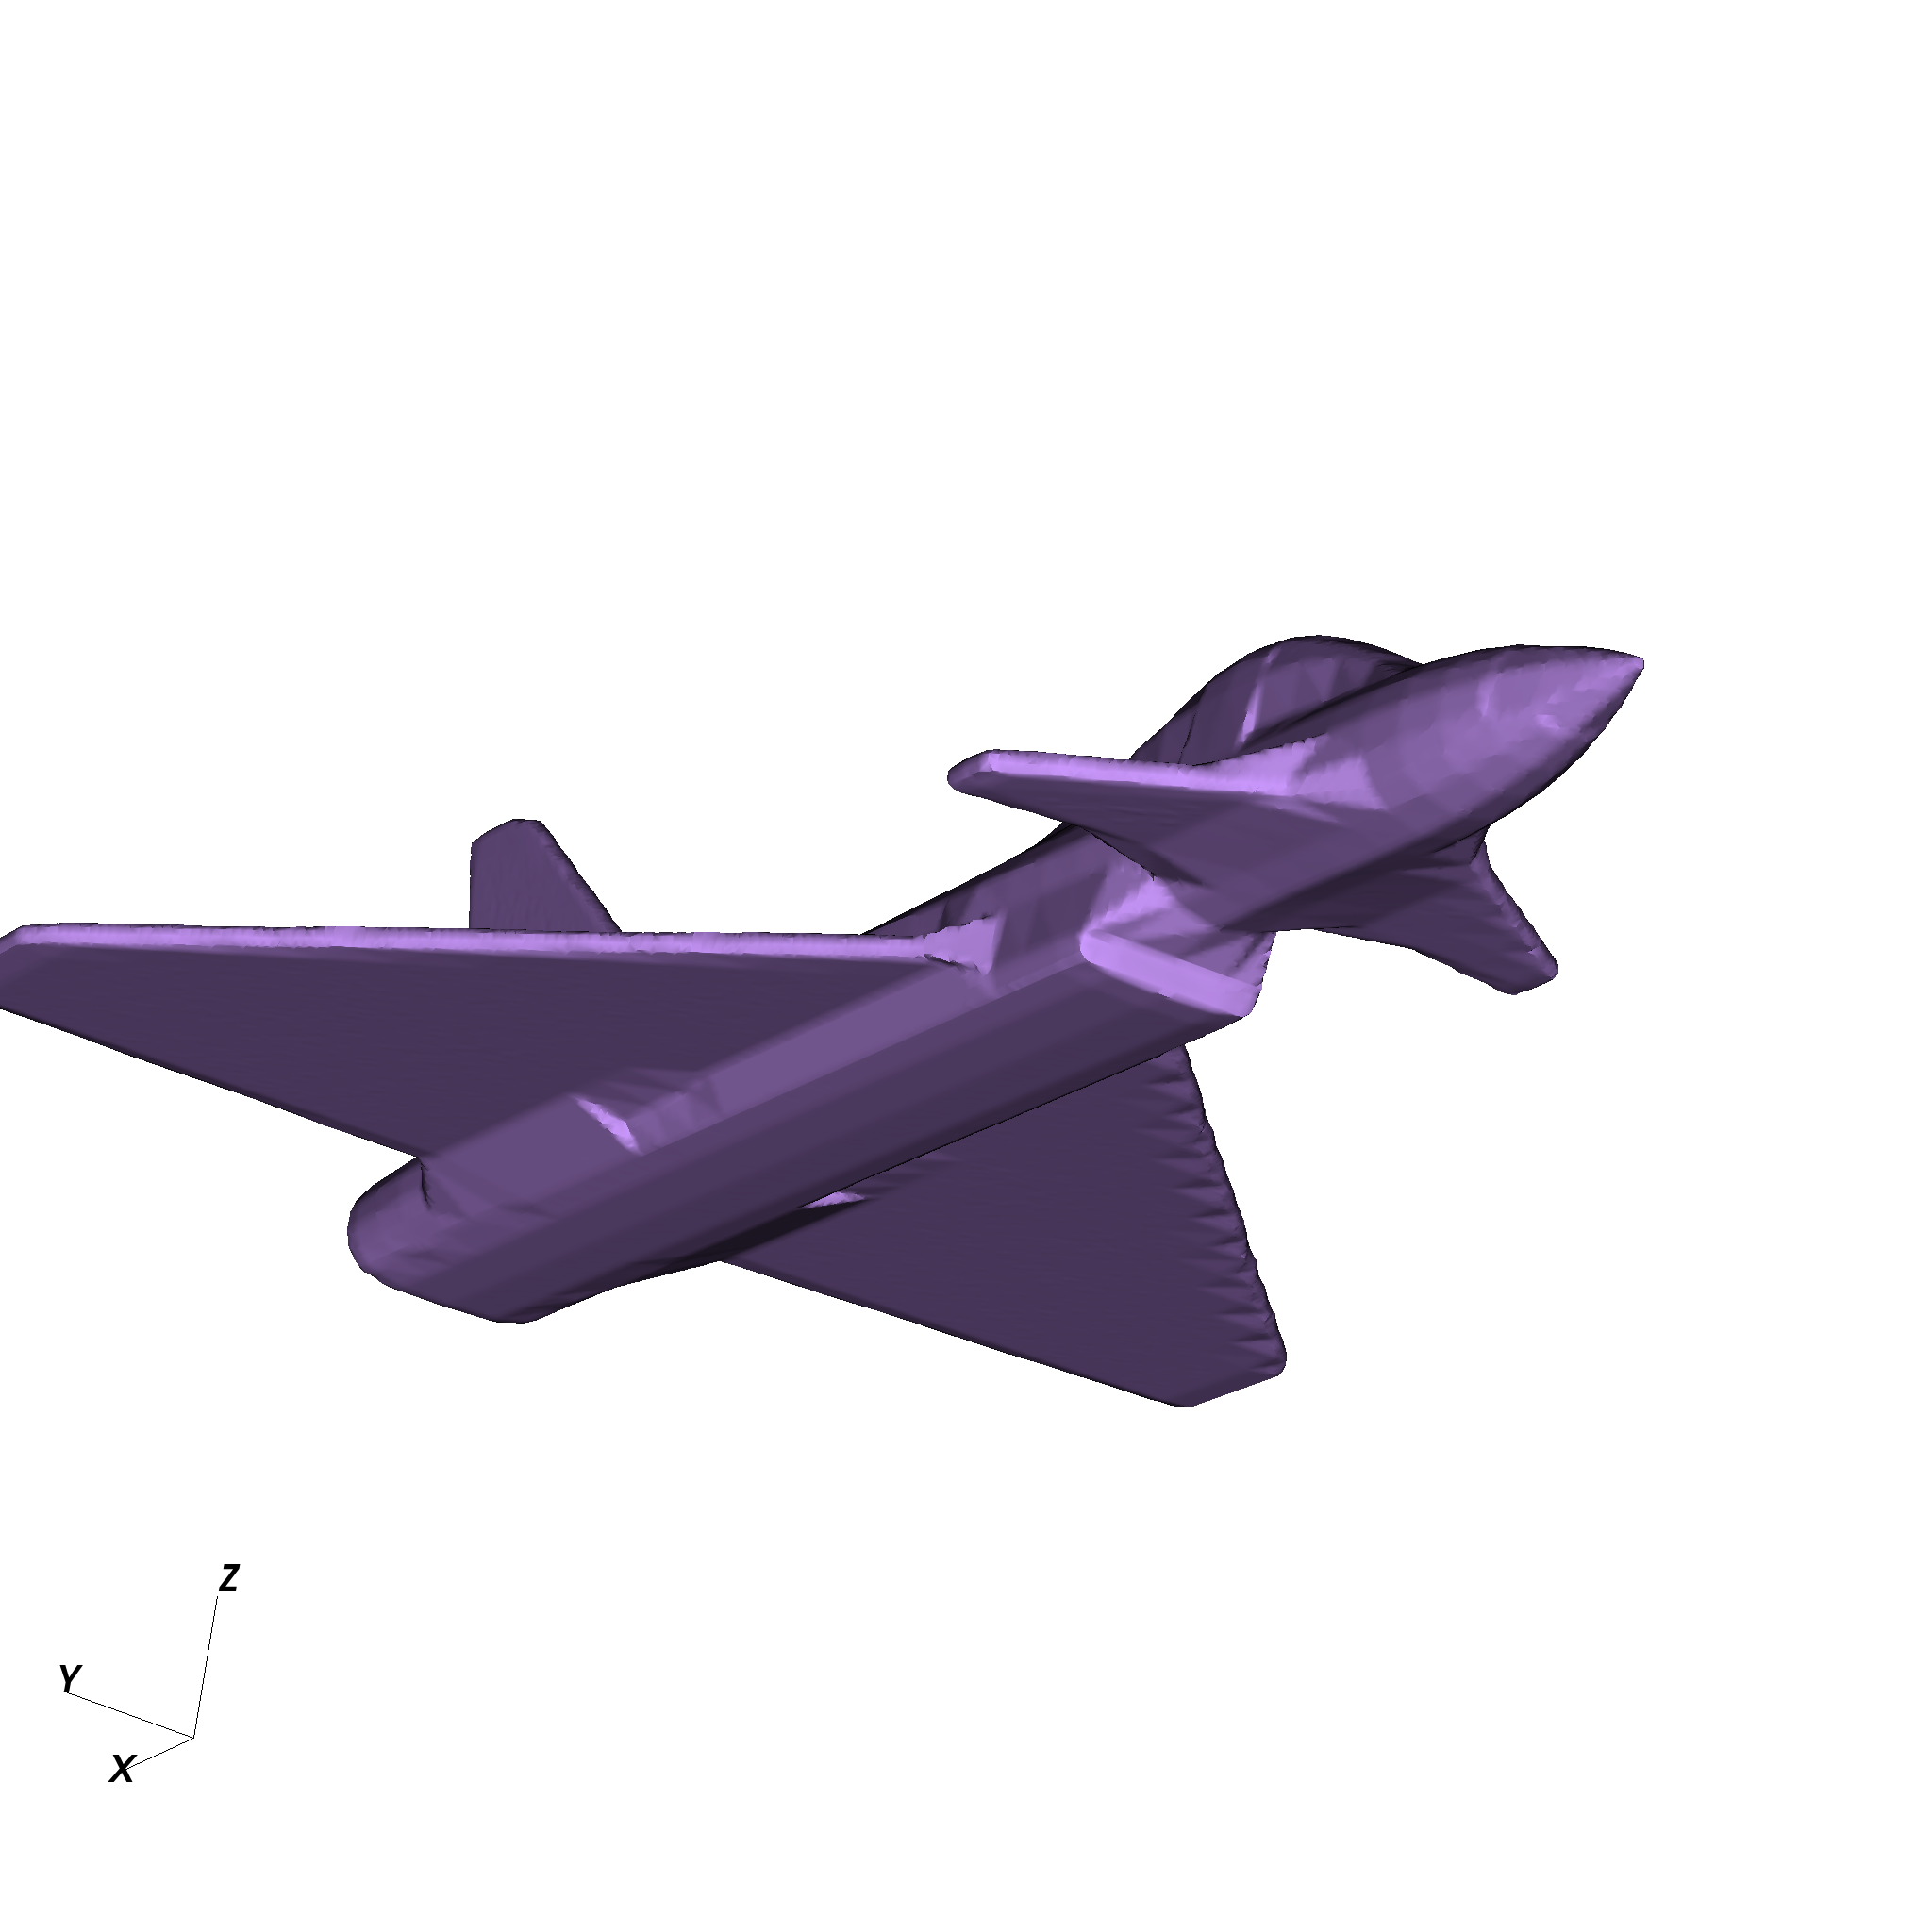
\includegraphics[width=\textwidth]{visit0016.png}
            \caption{}    
            \label{ef1}
        \end{subfigure}
        \hfill
        \begin{subfigure}[b]{0.475\textwidth}  
            \centering 
            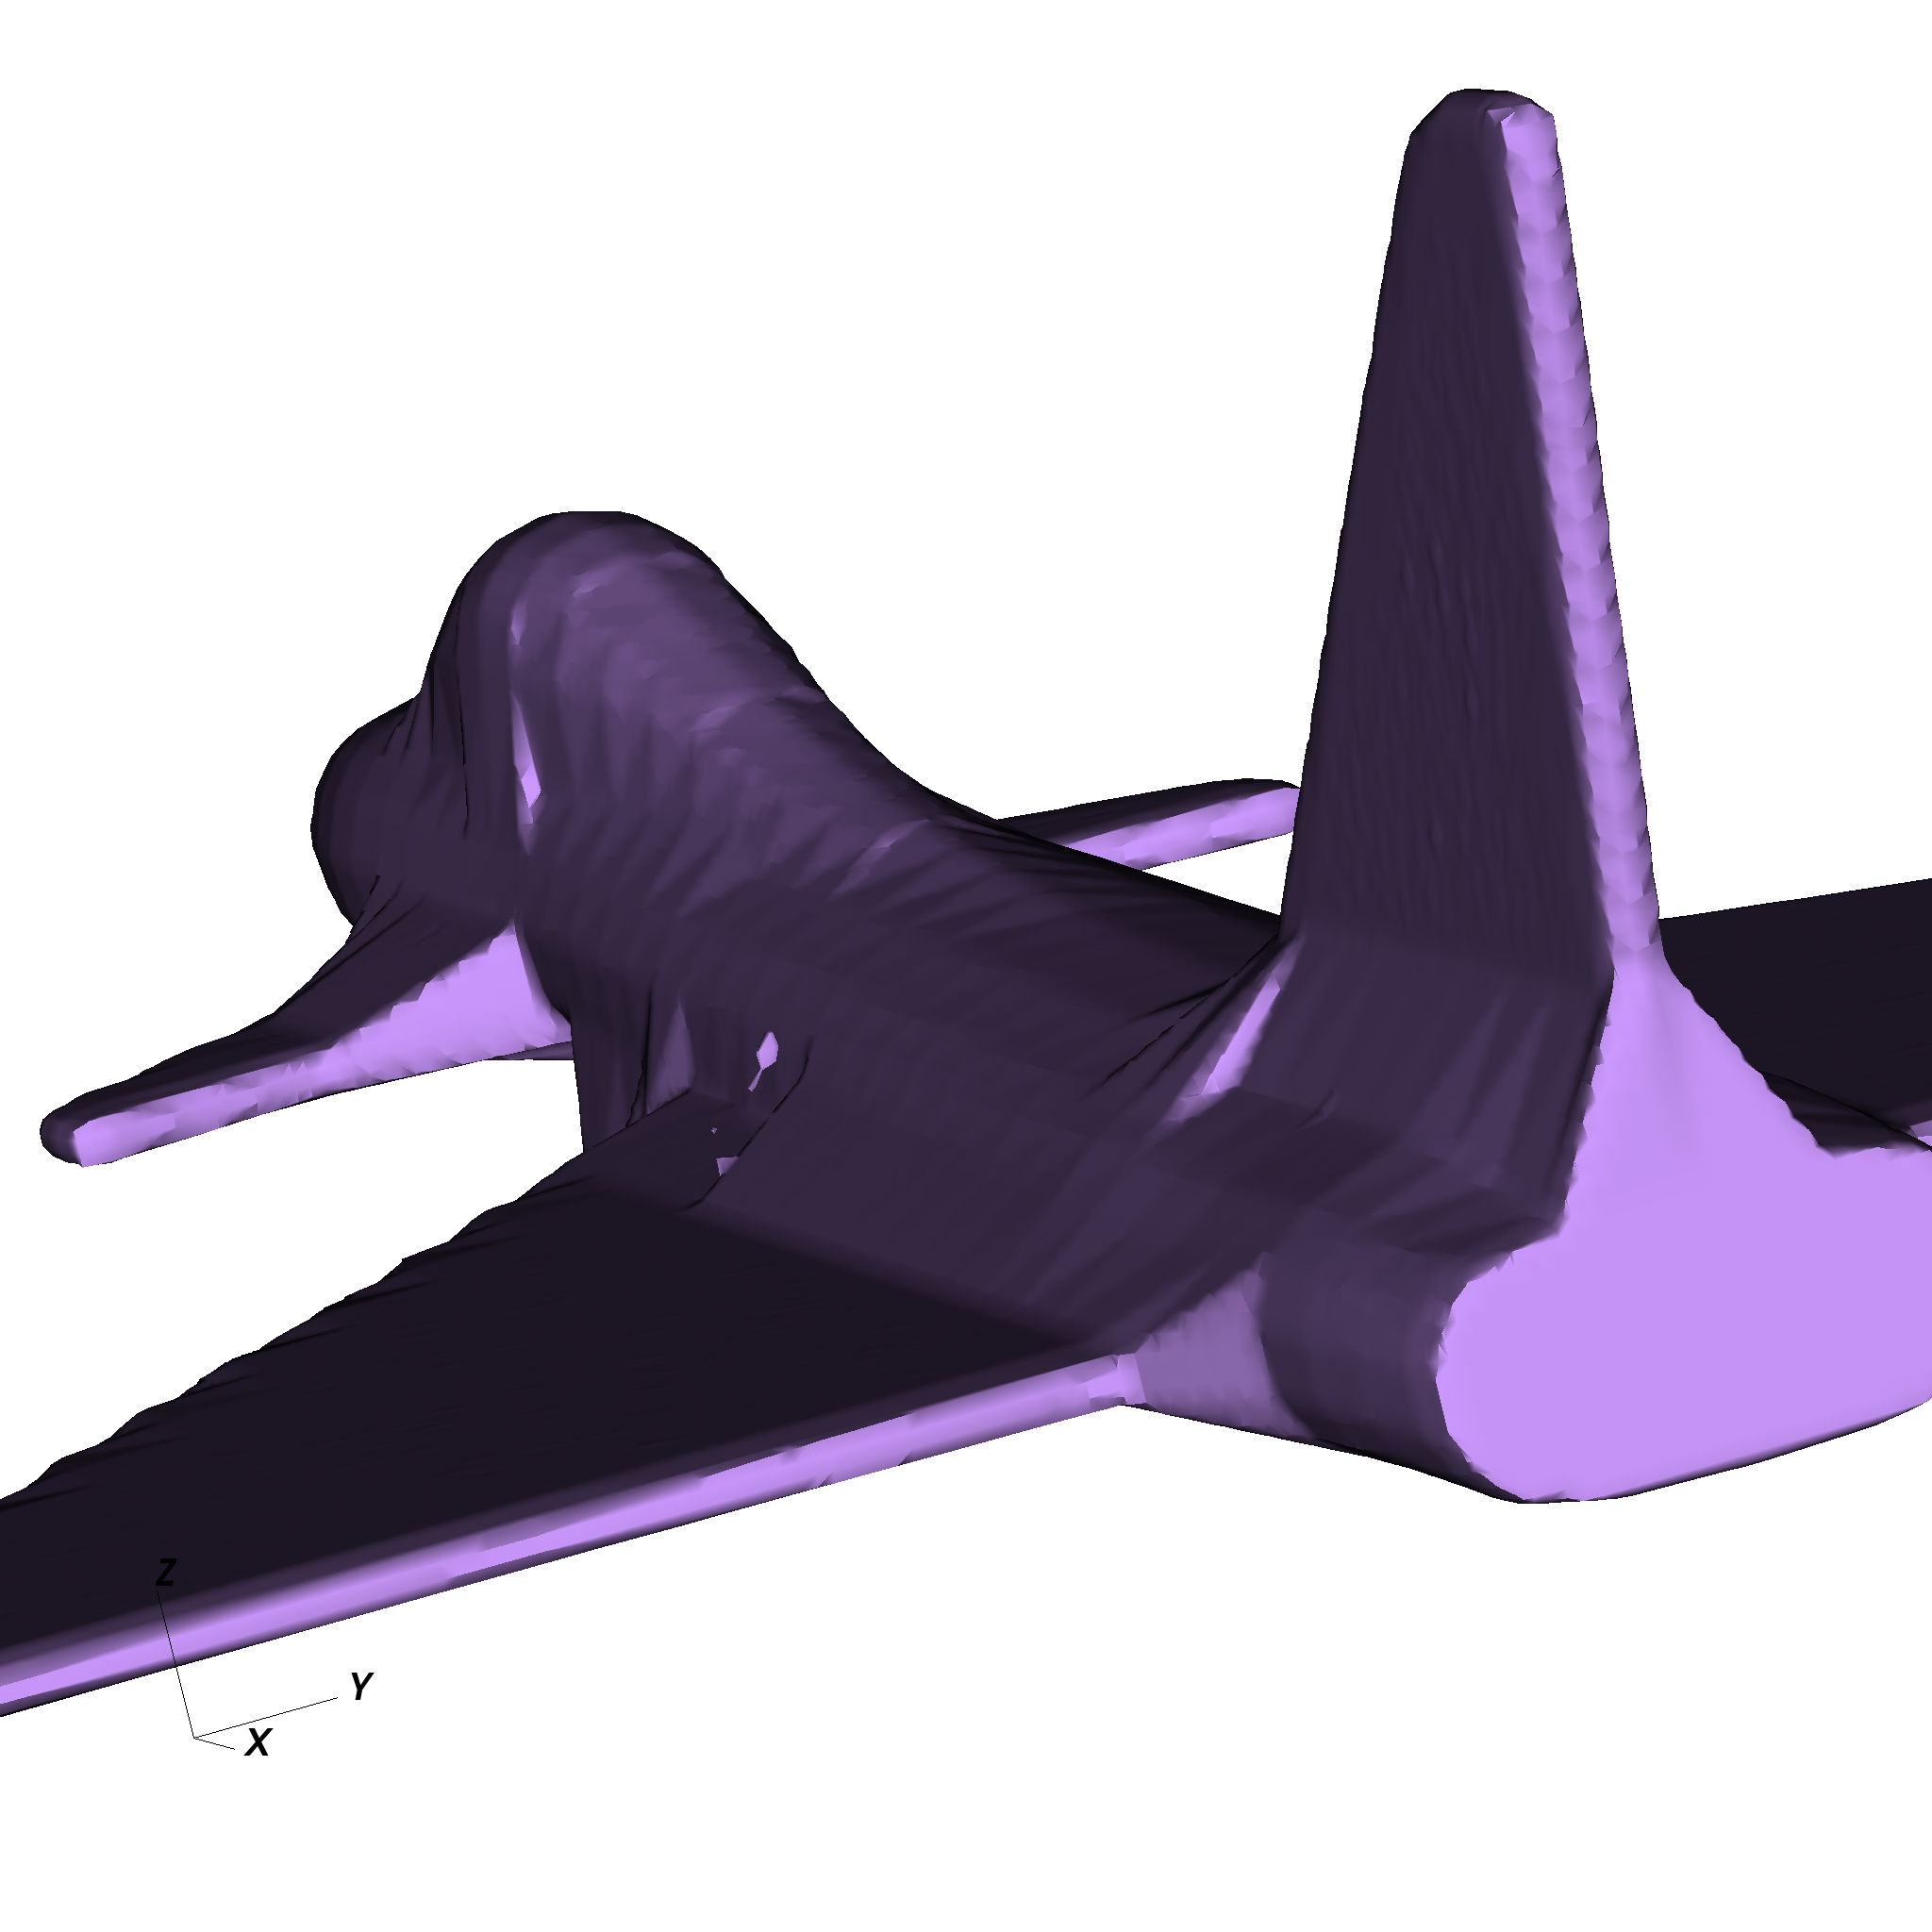
\includegraphics[width=\textwidth]{visit0013.png}
            \caption{}    
            \label{ef2}
        \end{subfigure}
        \vskip\baselineskip
        \begin{subfigure}[b]{0.475\textwidth}   
            \centering 
            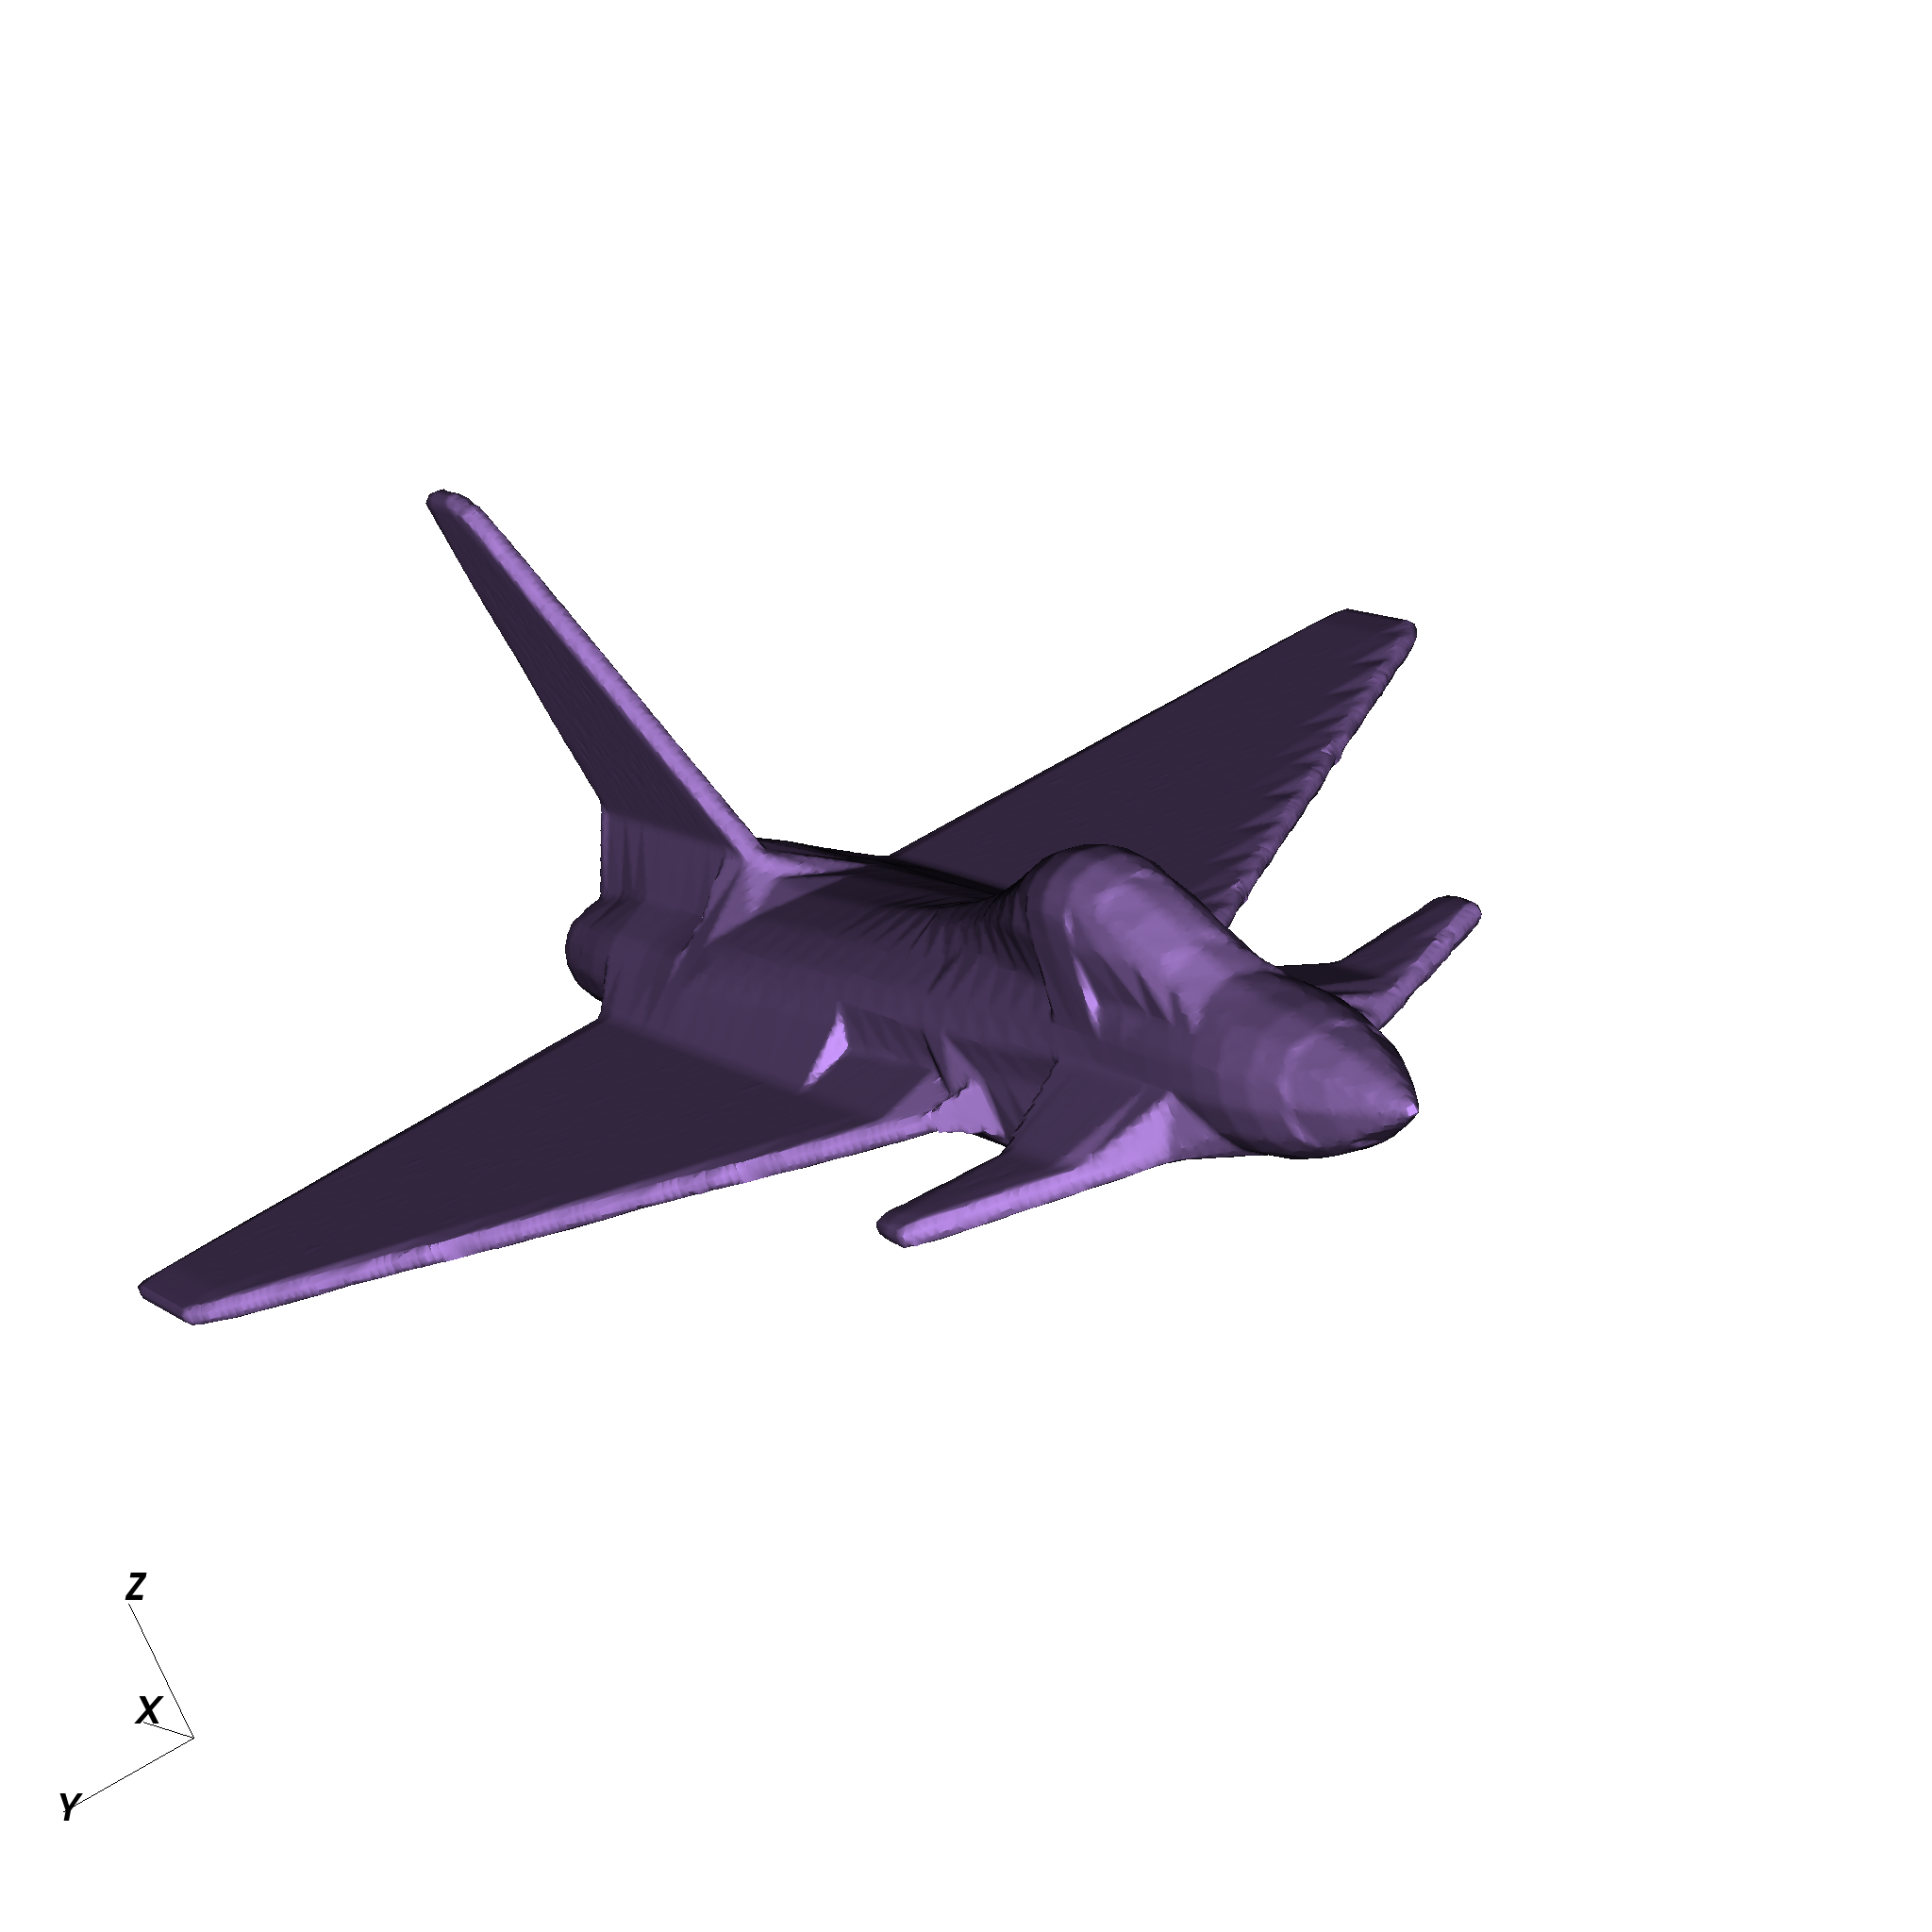
\includegraphics[width=\textwidth]{visit0015.png}
            \caption{}  
            \label{ef3}
        \end{subfigure}
        \quad
        \begin{subfigure}[b]{0.475\textwidth}   
            \centering 
            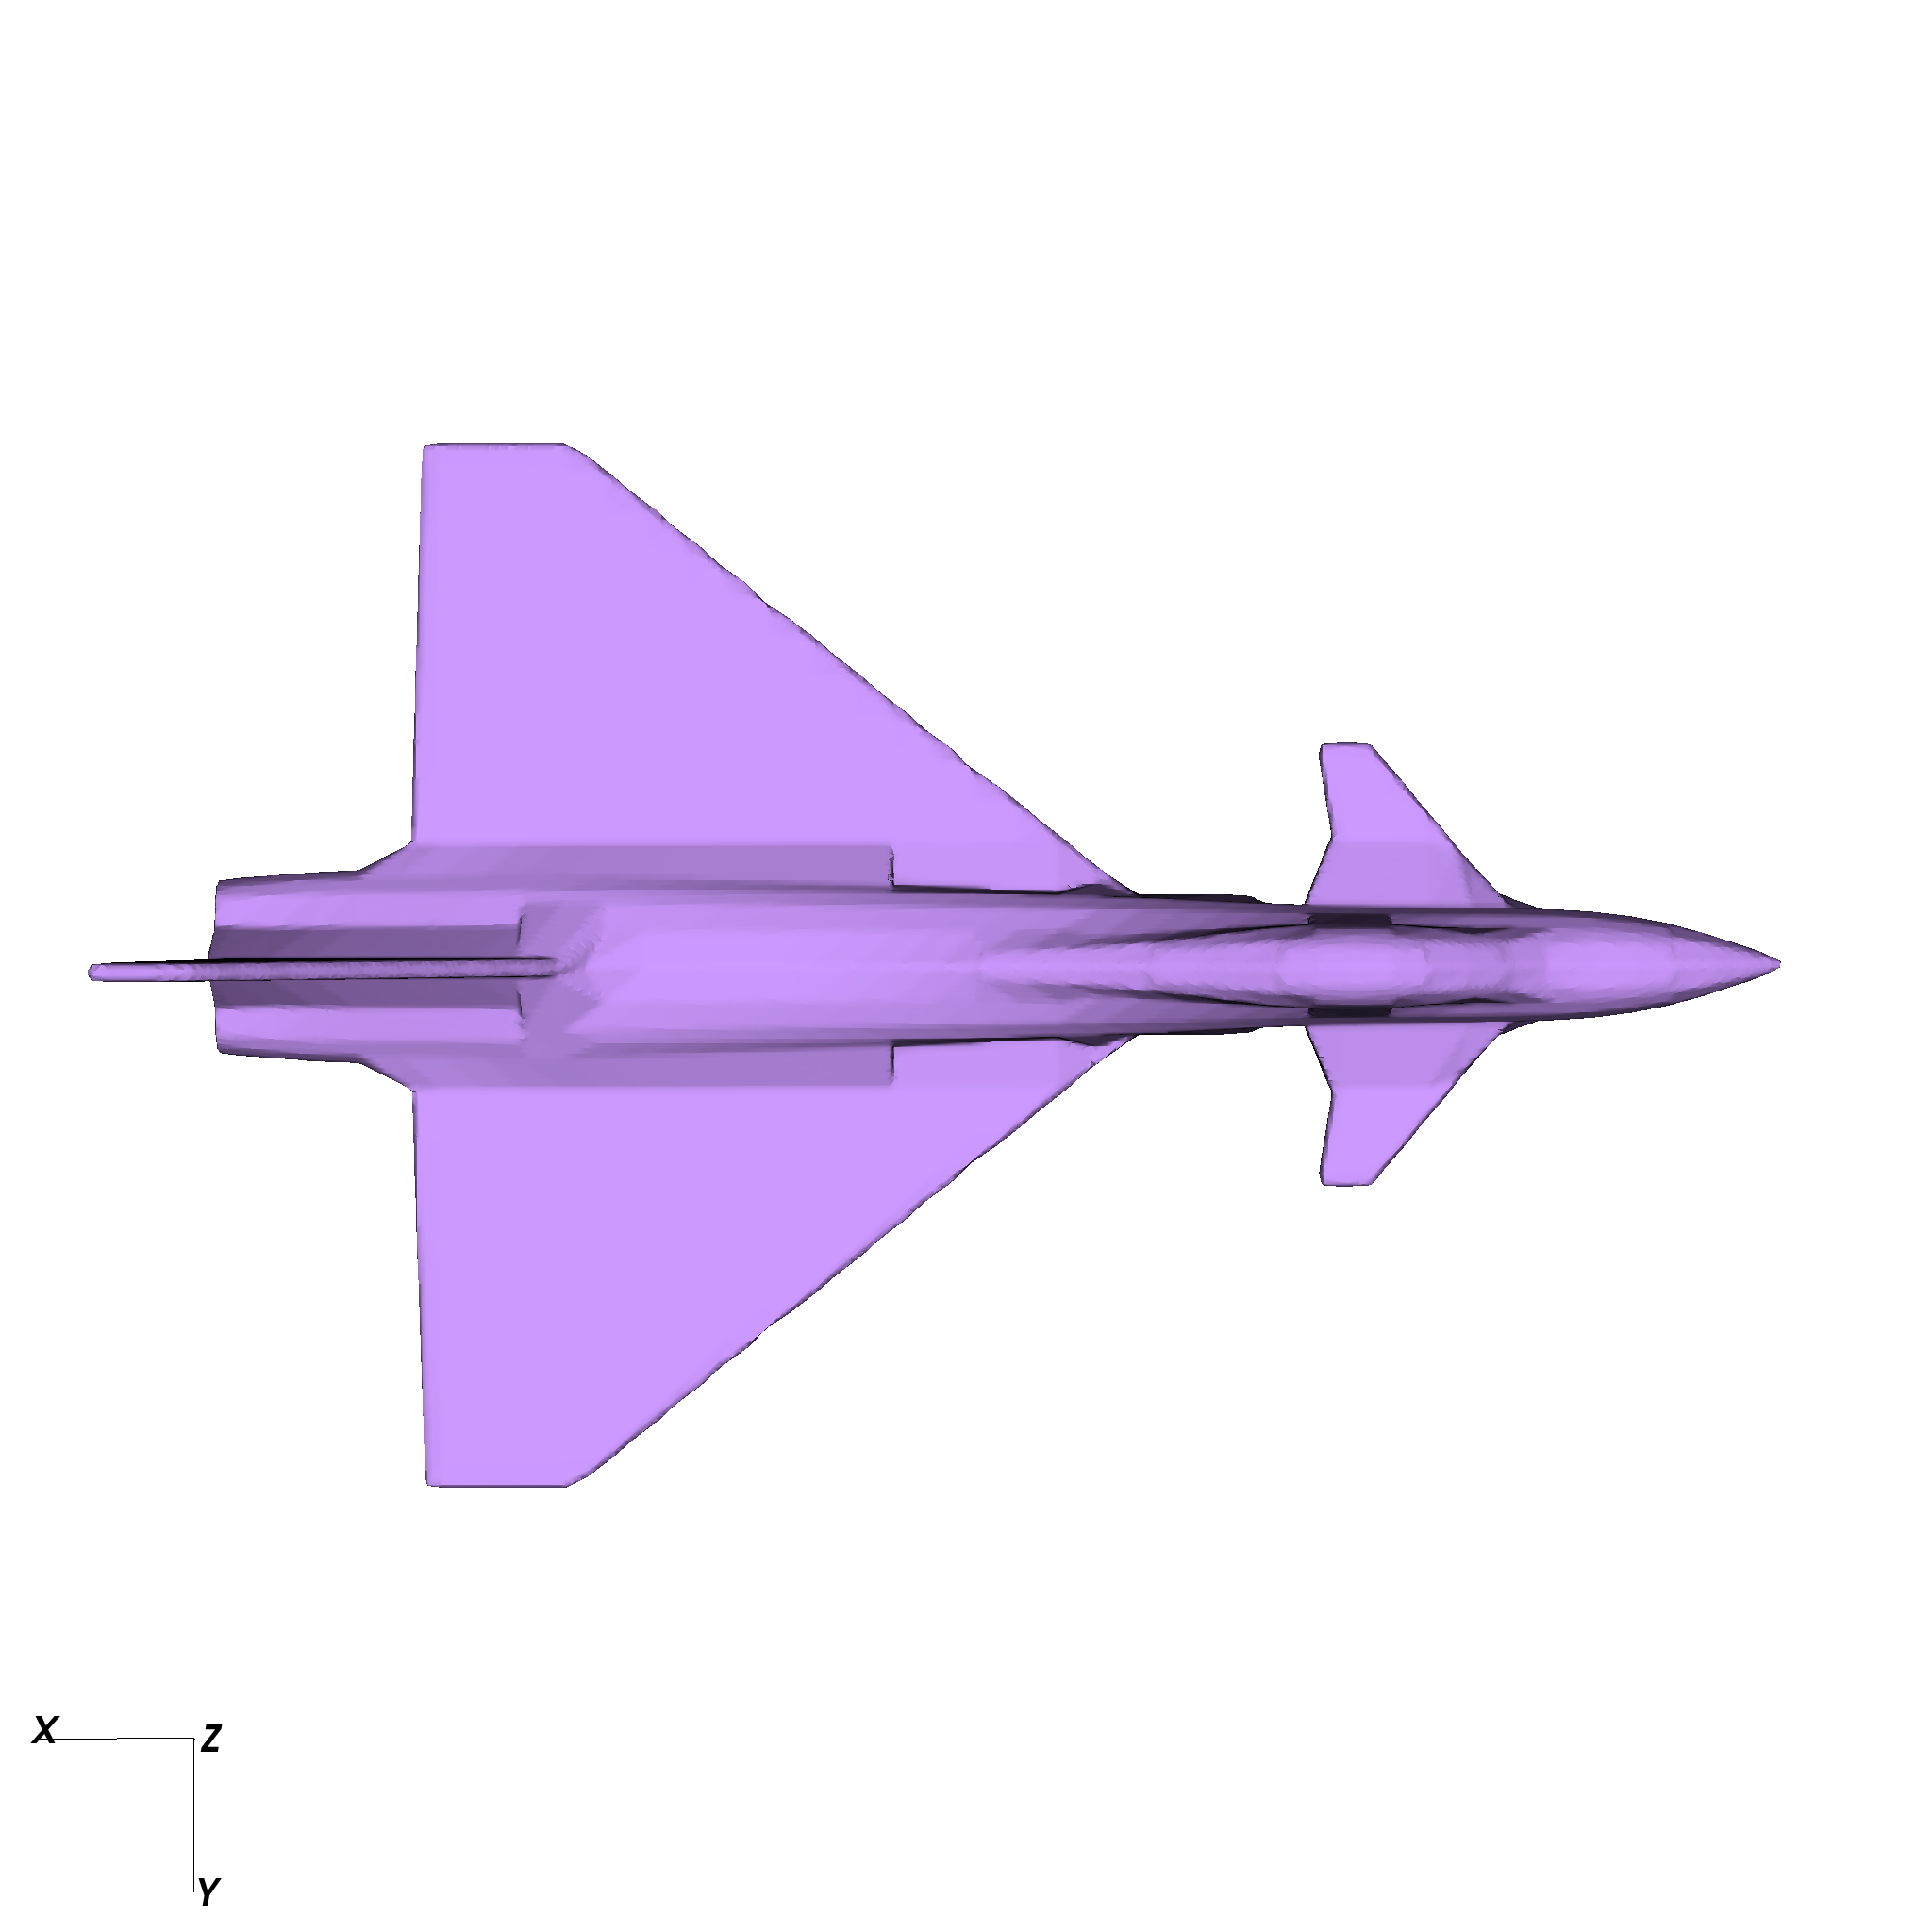
\includegraphics[width=\textwidth]{visit0012.png}
            \caption{}
            \label{ef4}
        \end{subfigure}
        \caption{The zero-level set of the signed distance function for the Eurofighter STL sampled on a $400^3$ mesh. There were $4\times 10^6$ marker particles seeded over the triangulated surface. The code ran in $\sim$5 minutes. In (b) a small artefact is visible over the left wing- this is a small region erroneously computed to be inside the plane due to part of one triangle protruding from
        the surface.}
        \label{EF}
\end{figure*}

\begin{figure*}
\centering
        \begin{subfigure}[b]{0.475\textwidth}
            \centering
            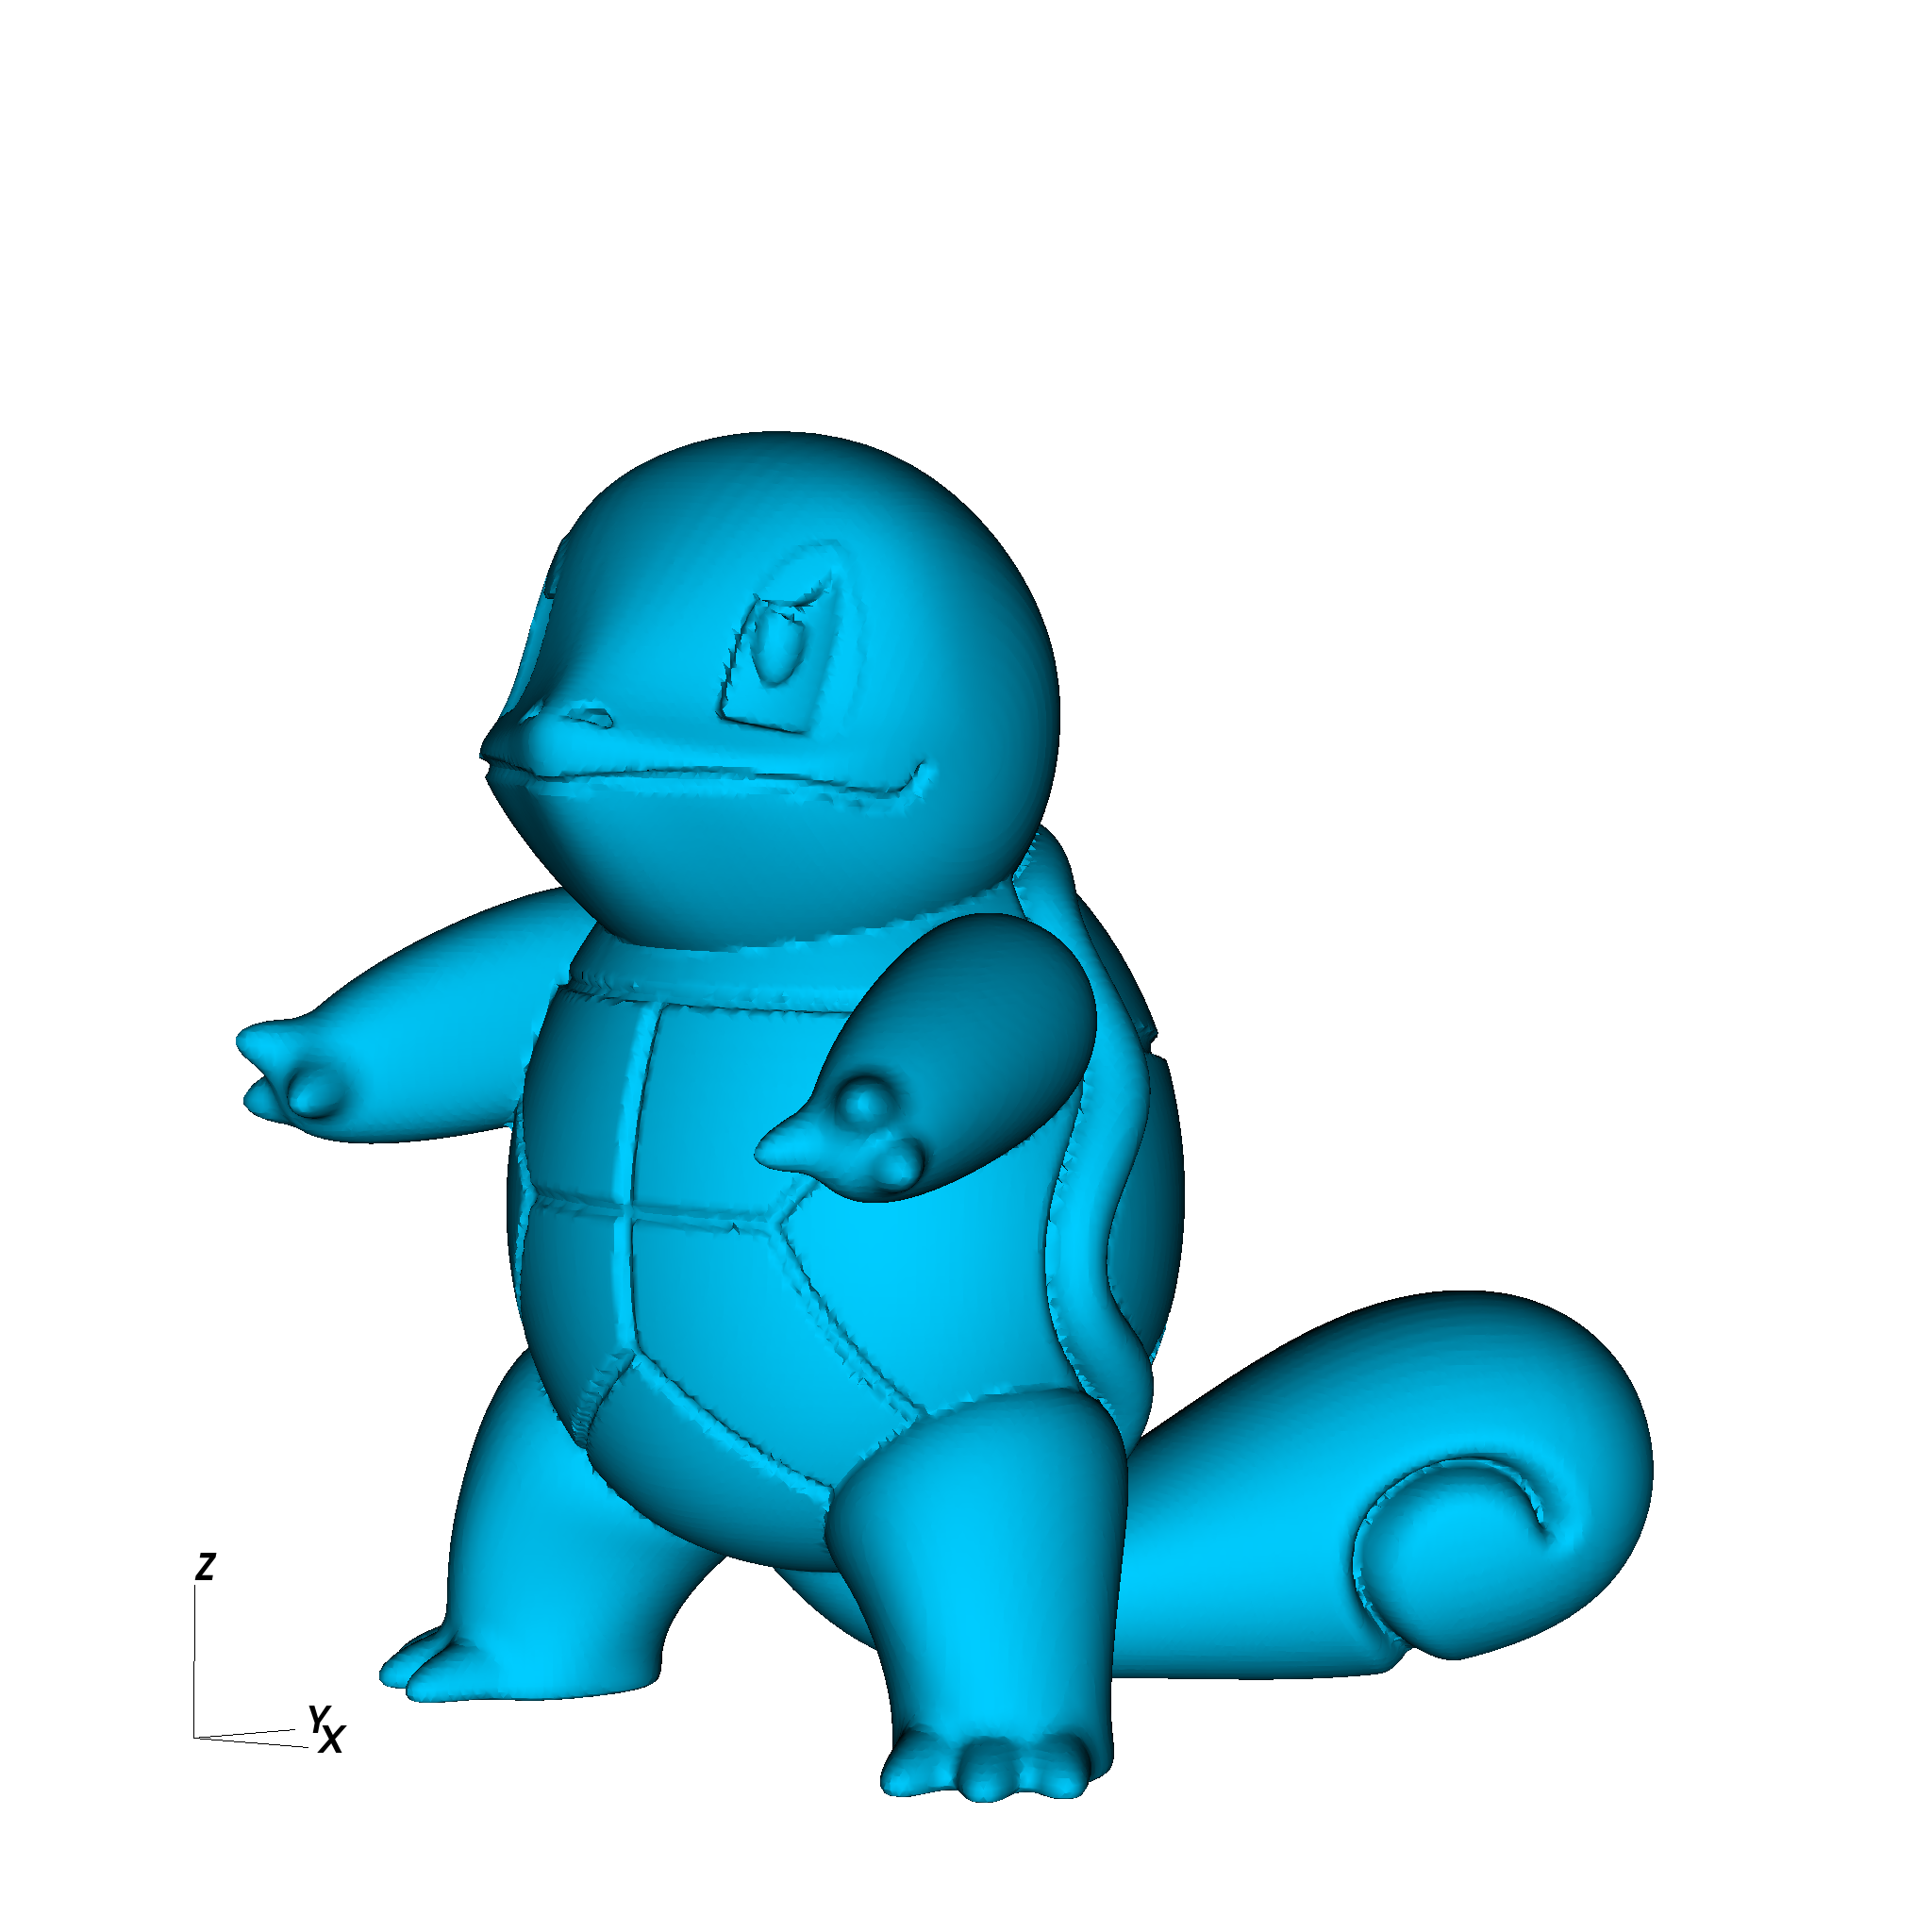
\includegraphics[width=\textwidth]{visit0018.png}
            \caption{}    
            \label{ef1}
        \end{subfigure}
        \hfill
        \begin{subfigure}[b]{0.475\textwidth}  
            \centering 
            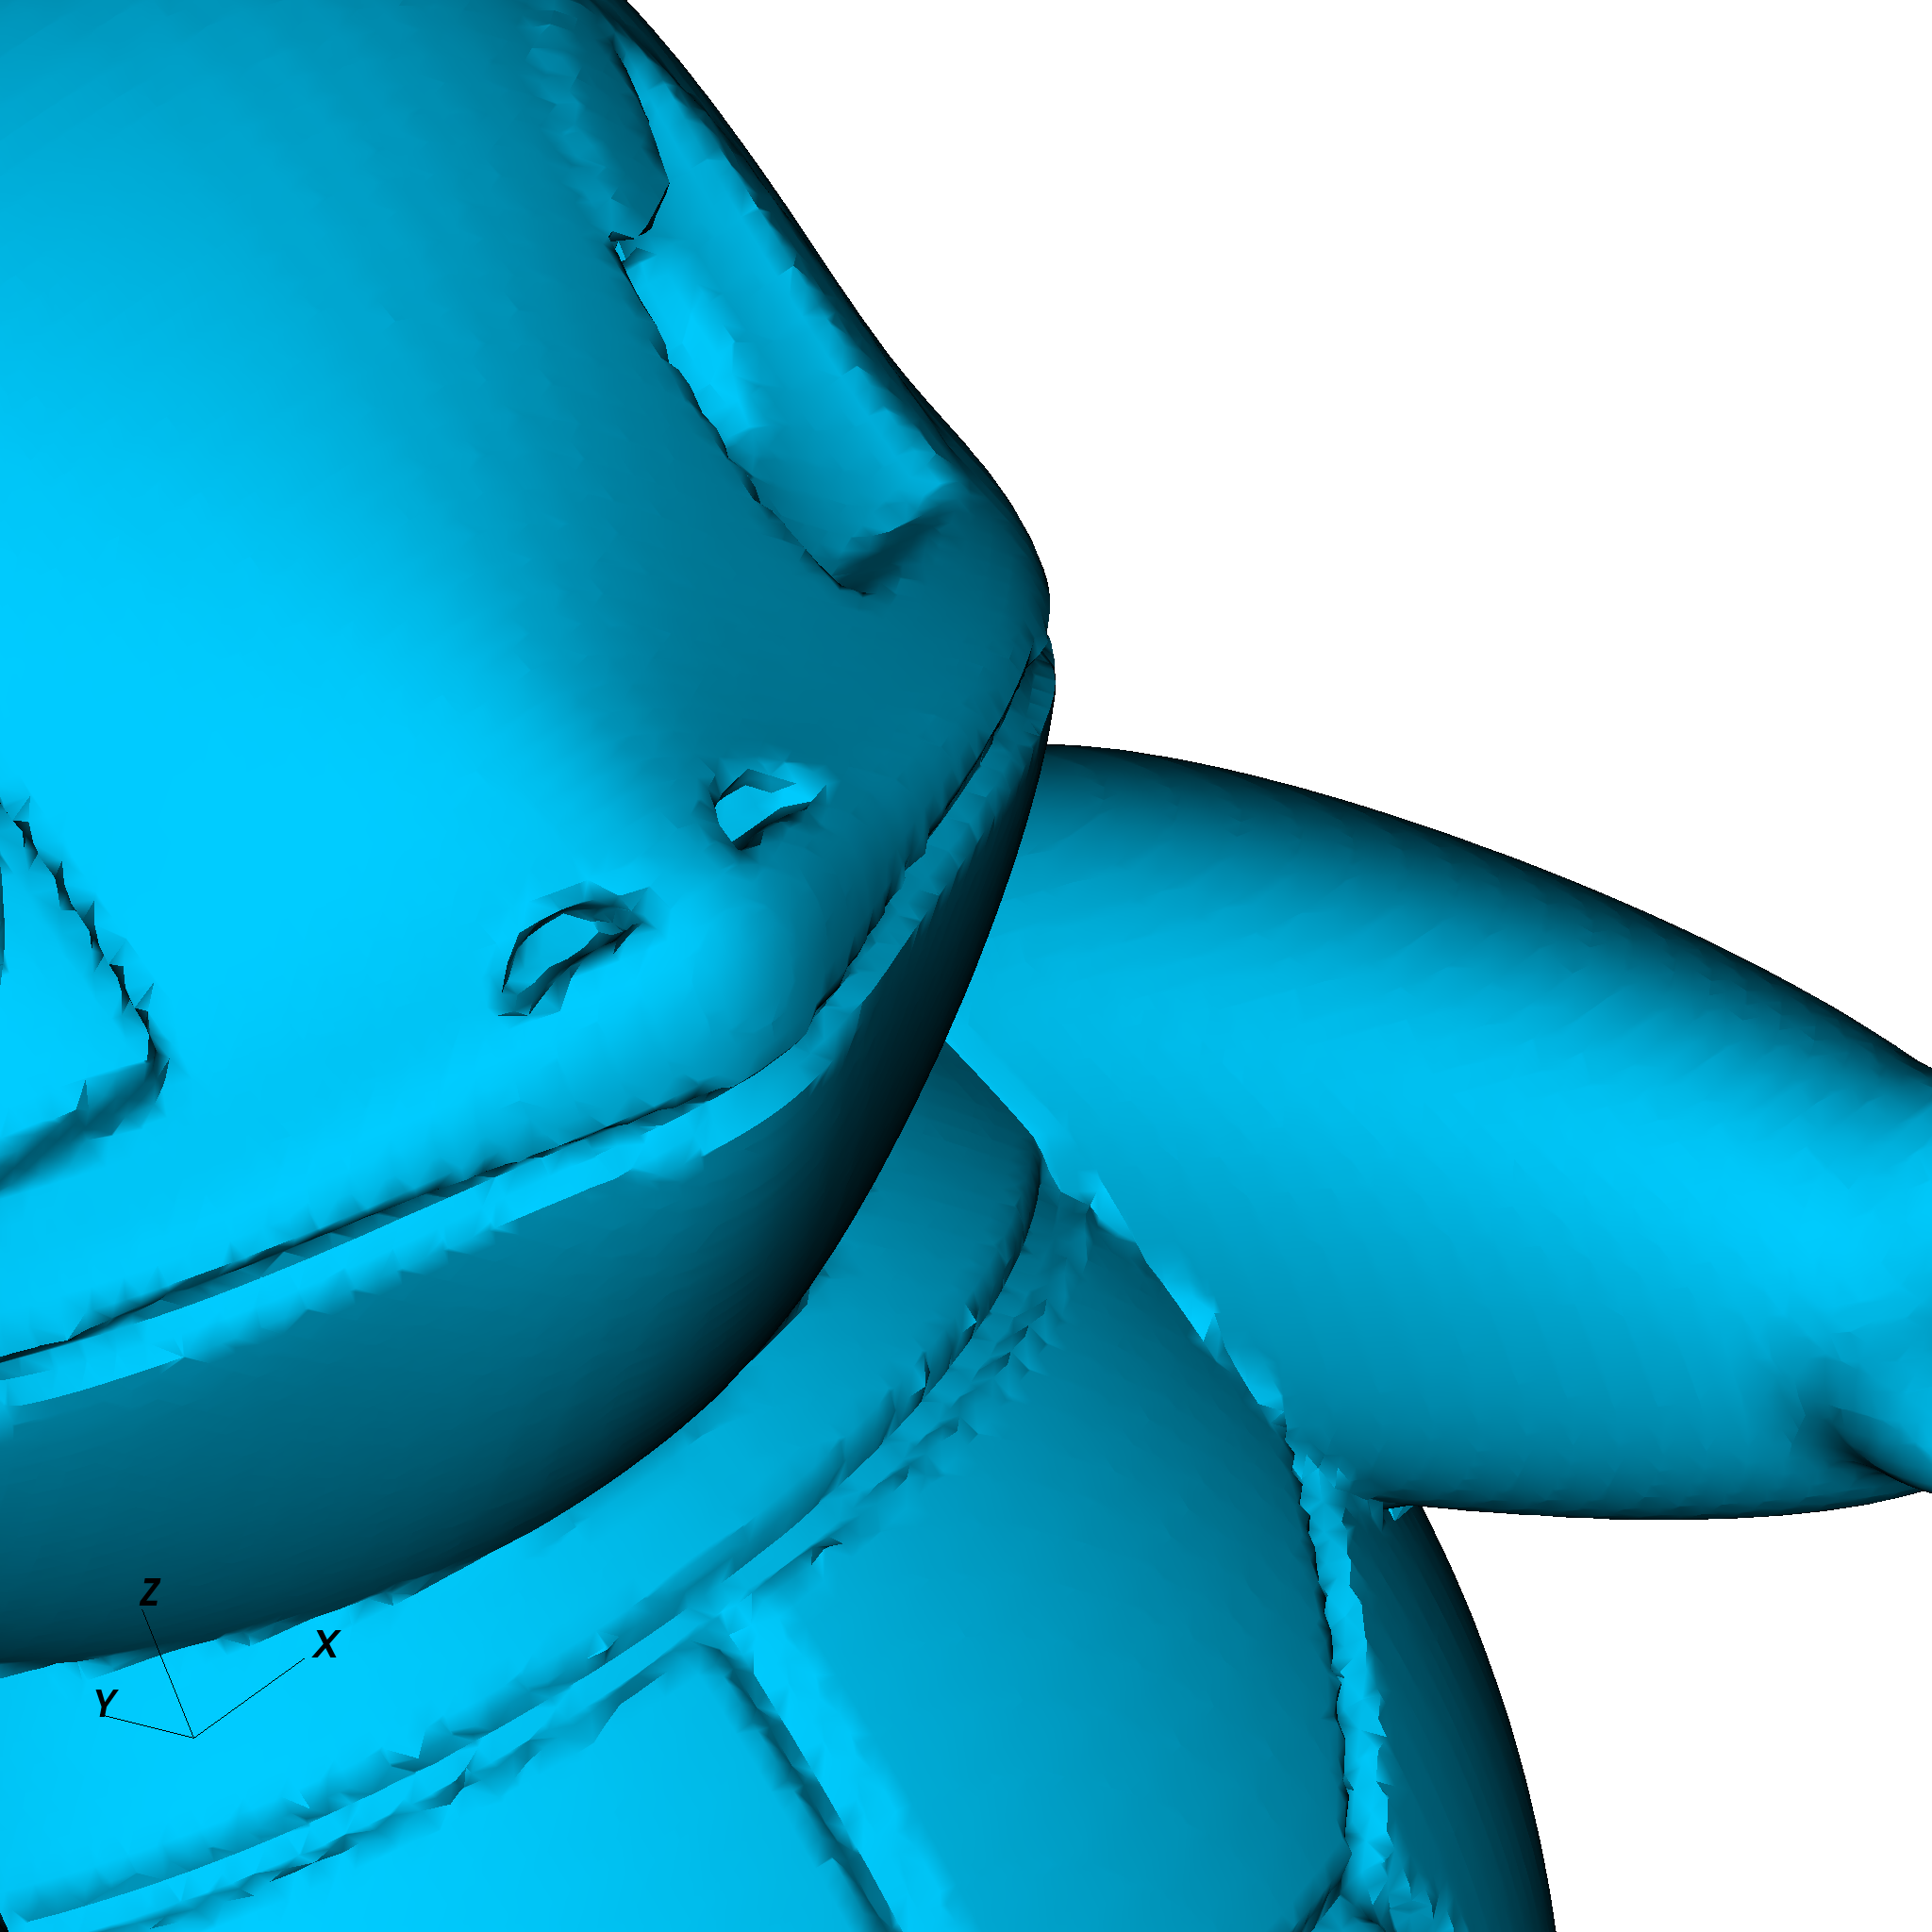
\includegraphics[width=\textwidth]{visit0019.png}
            \caption{}    
            \label{ef2}
        \end{subfigure}
        \vskip\baselineskip
        \begin{subfigure}[b]{0.475\textwidth}   
            \centering 
            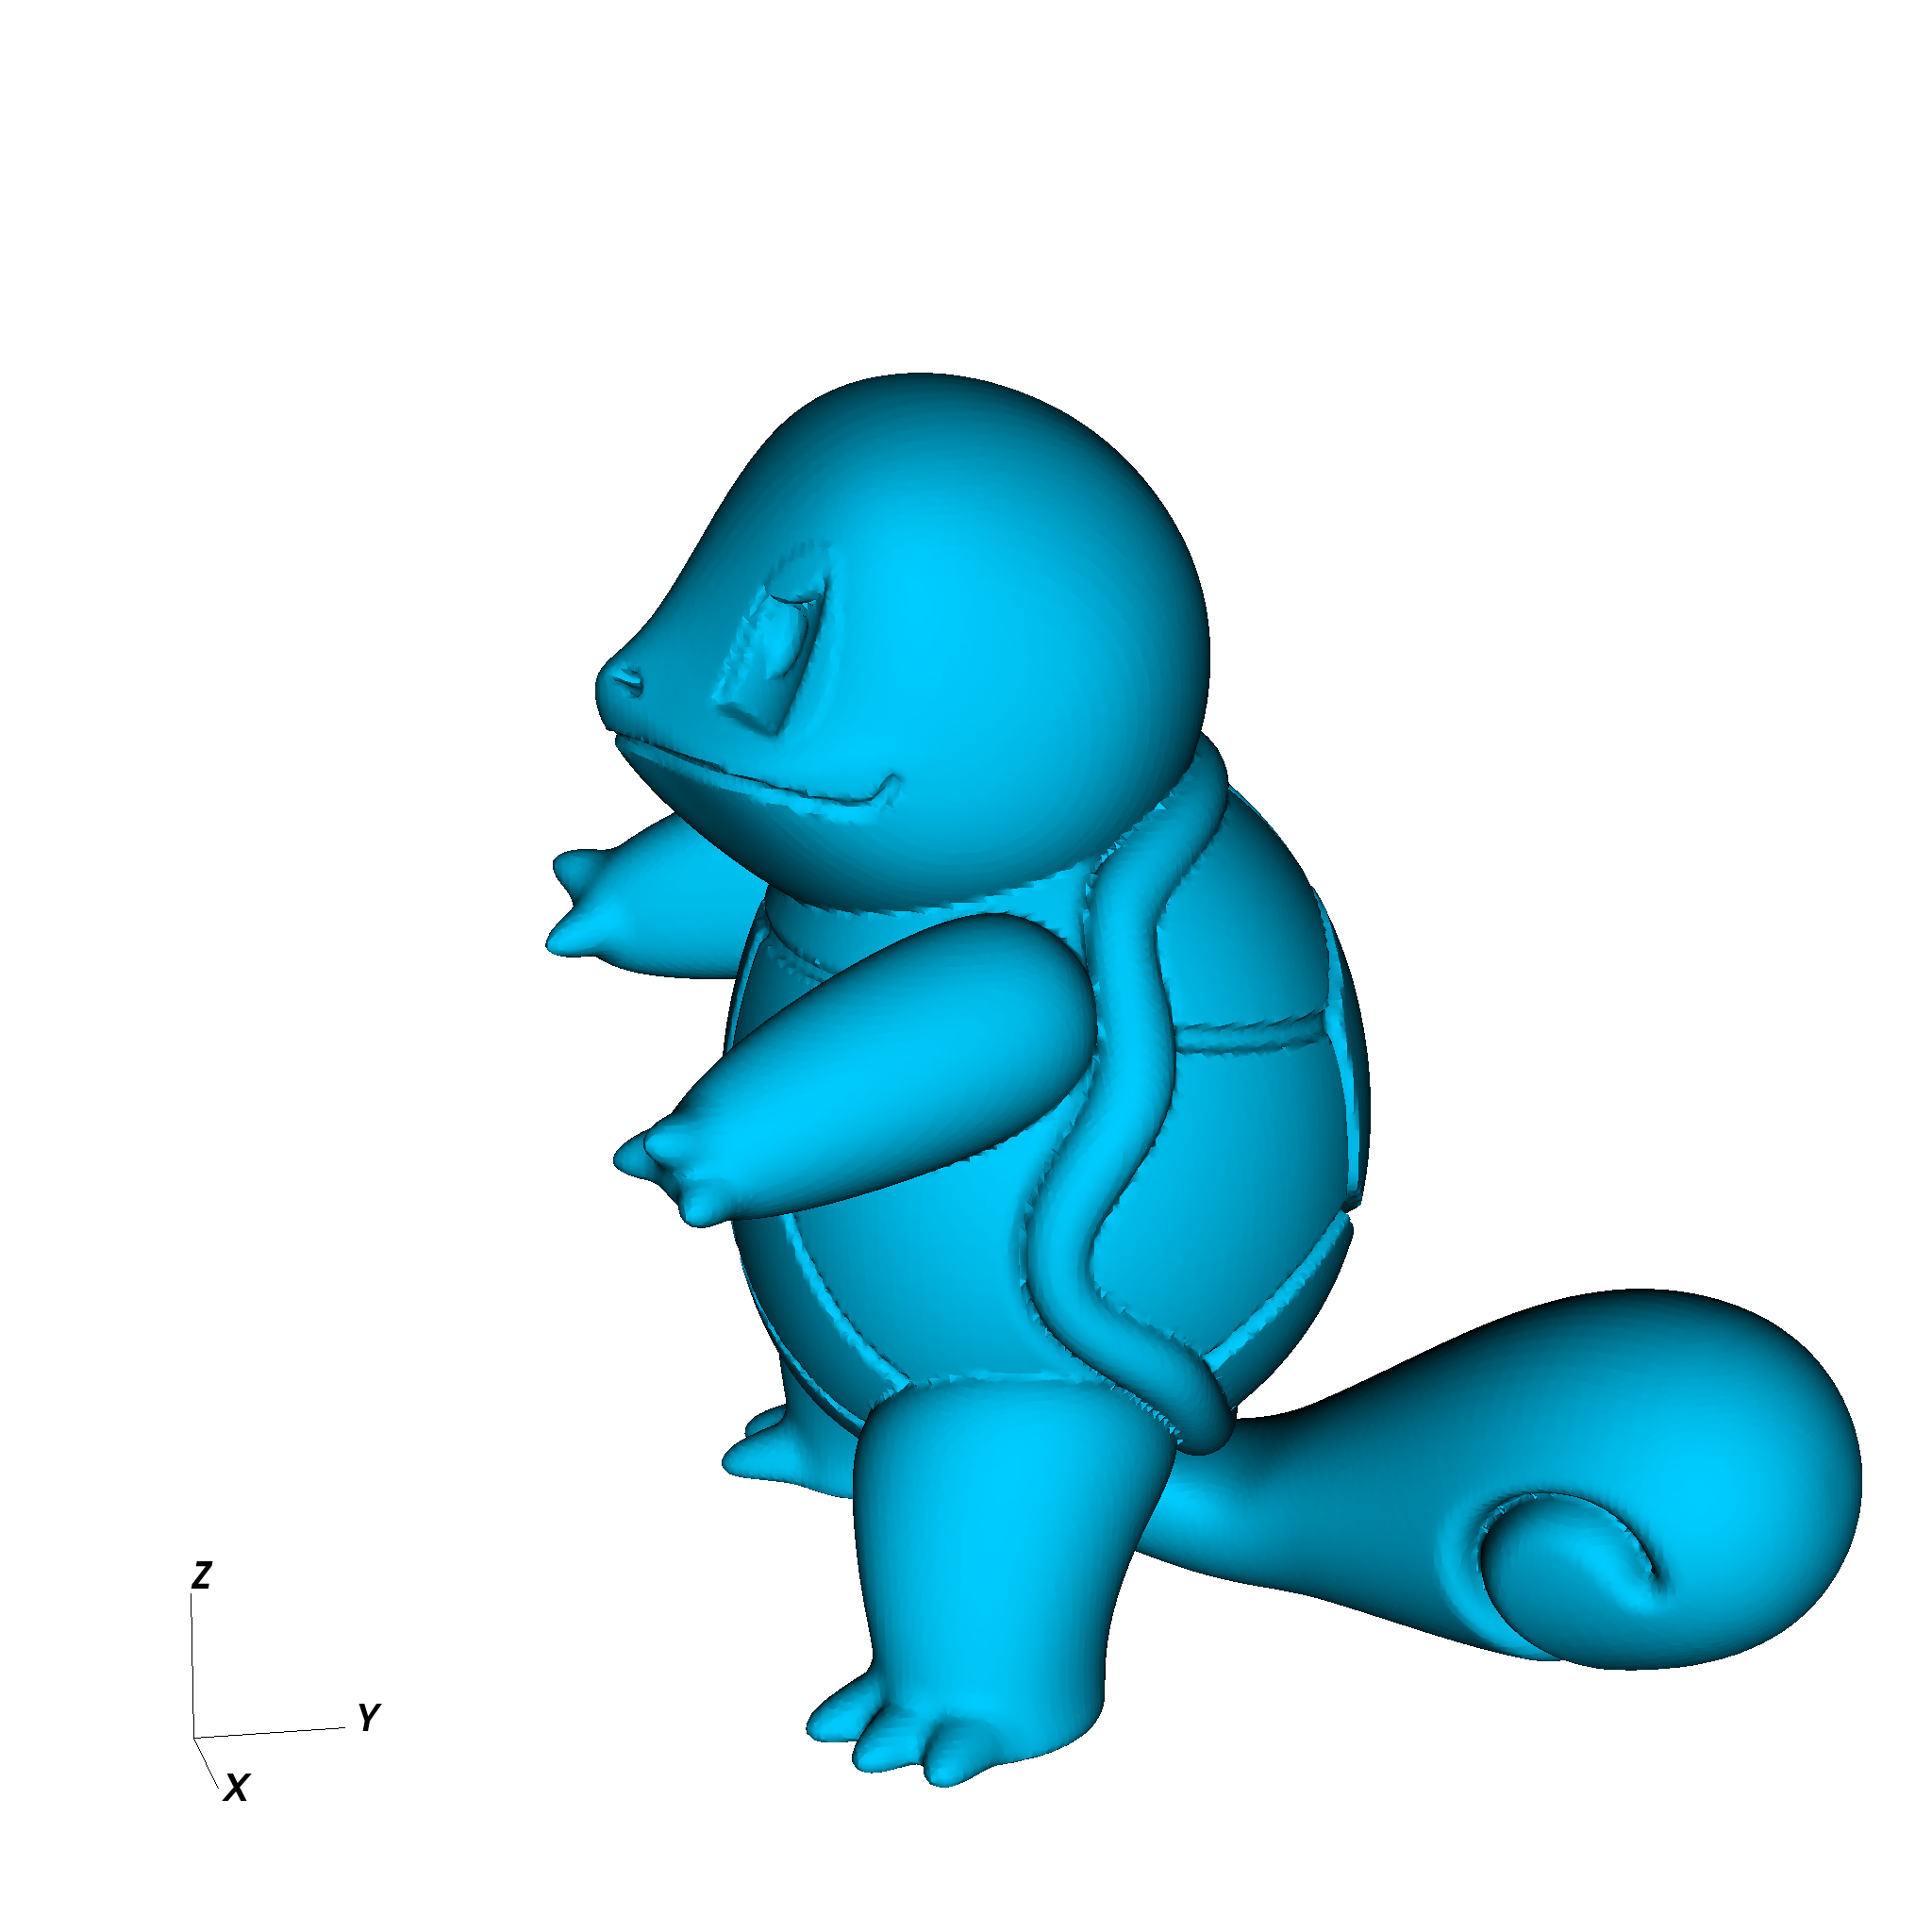
\includegraphics[width=\textwidth]{visit0020.png}
            \caption{}  
            \label{ef3}
        \end{subfigure}
        \quad
        \begin{subfigure}[b]{0.475\textwidth}   
            \centering 
            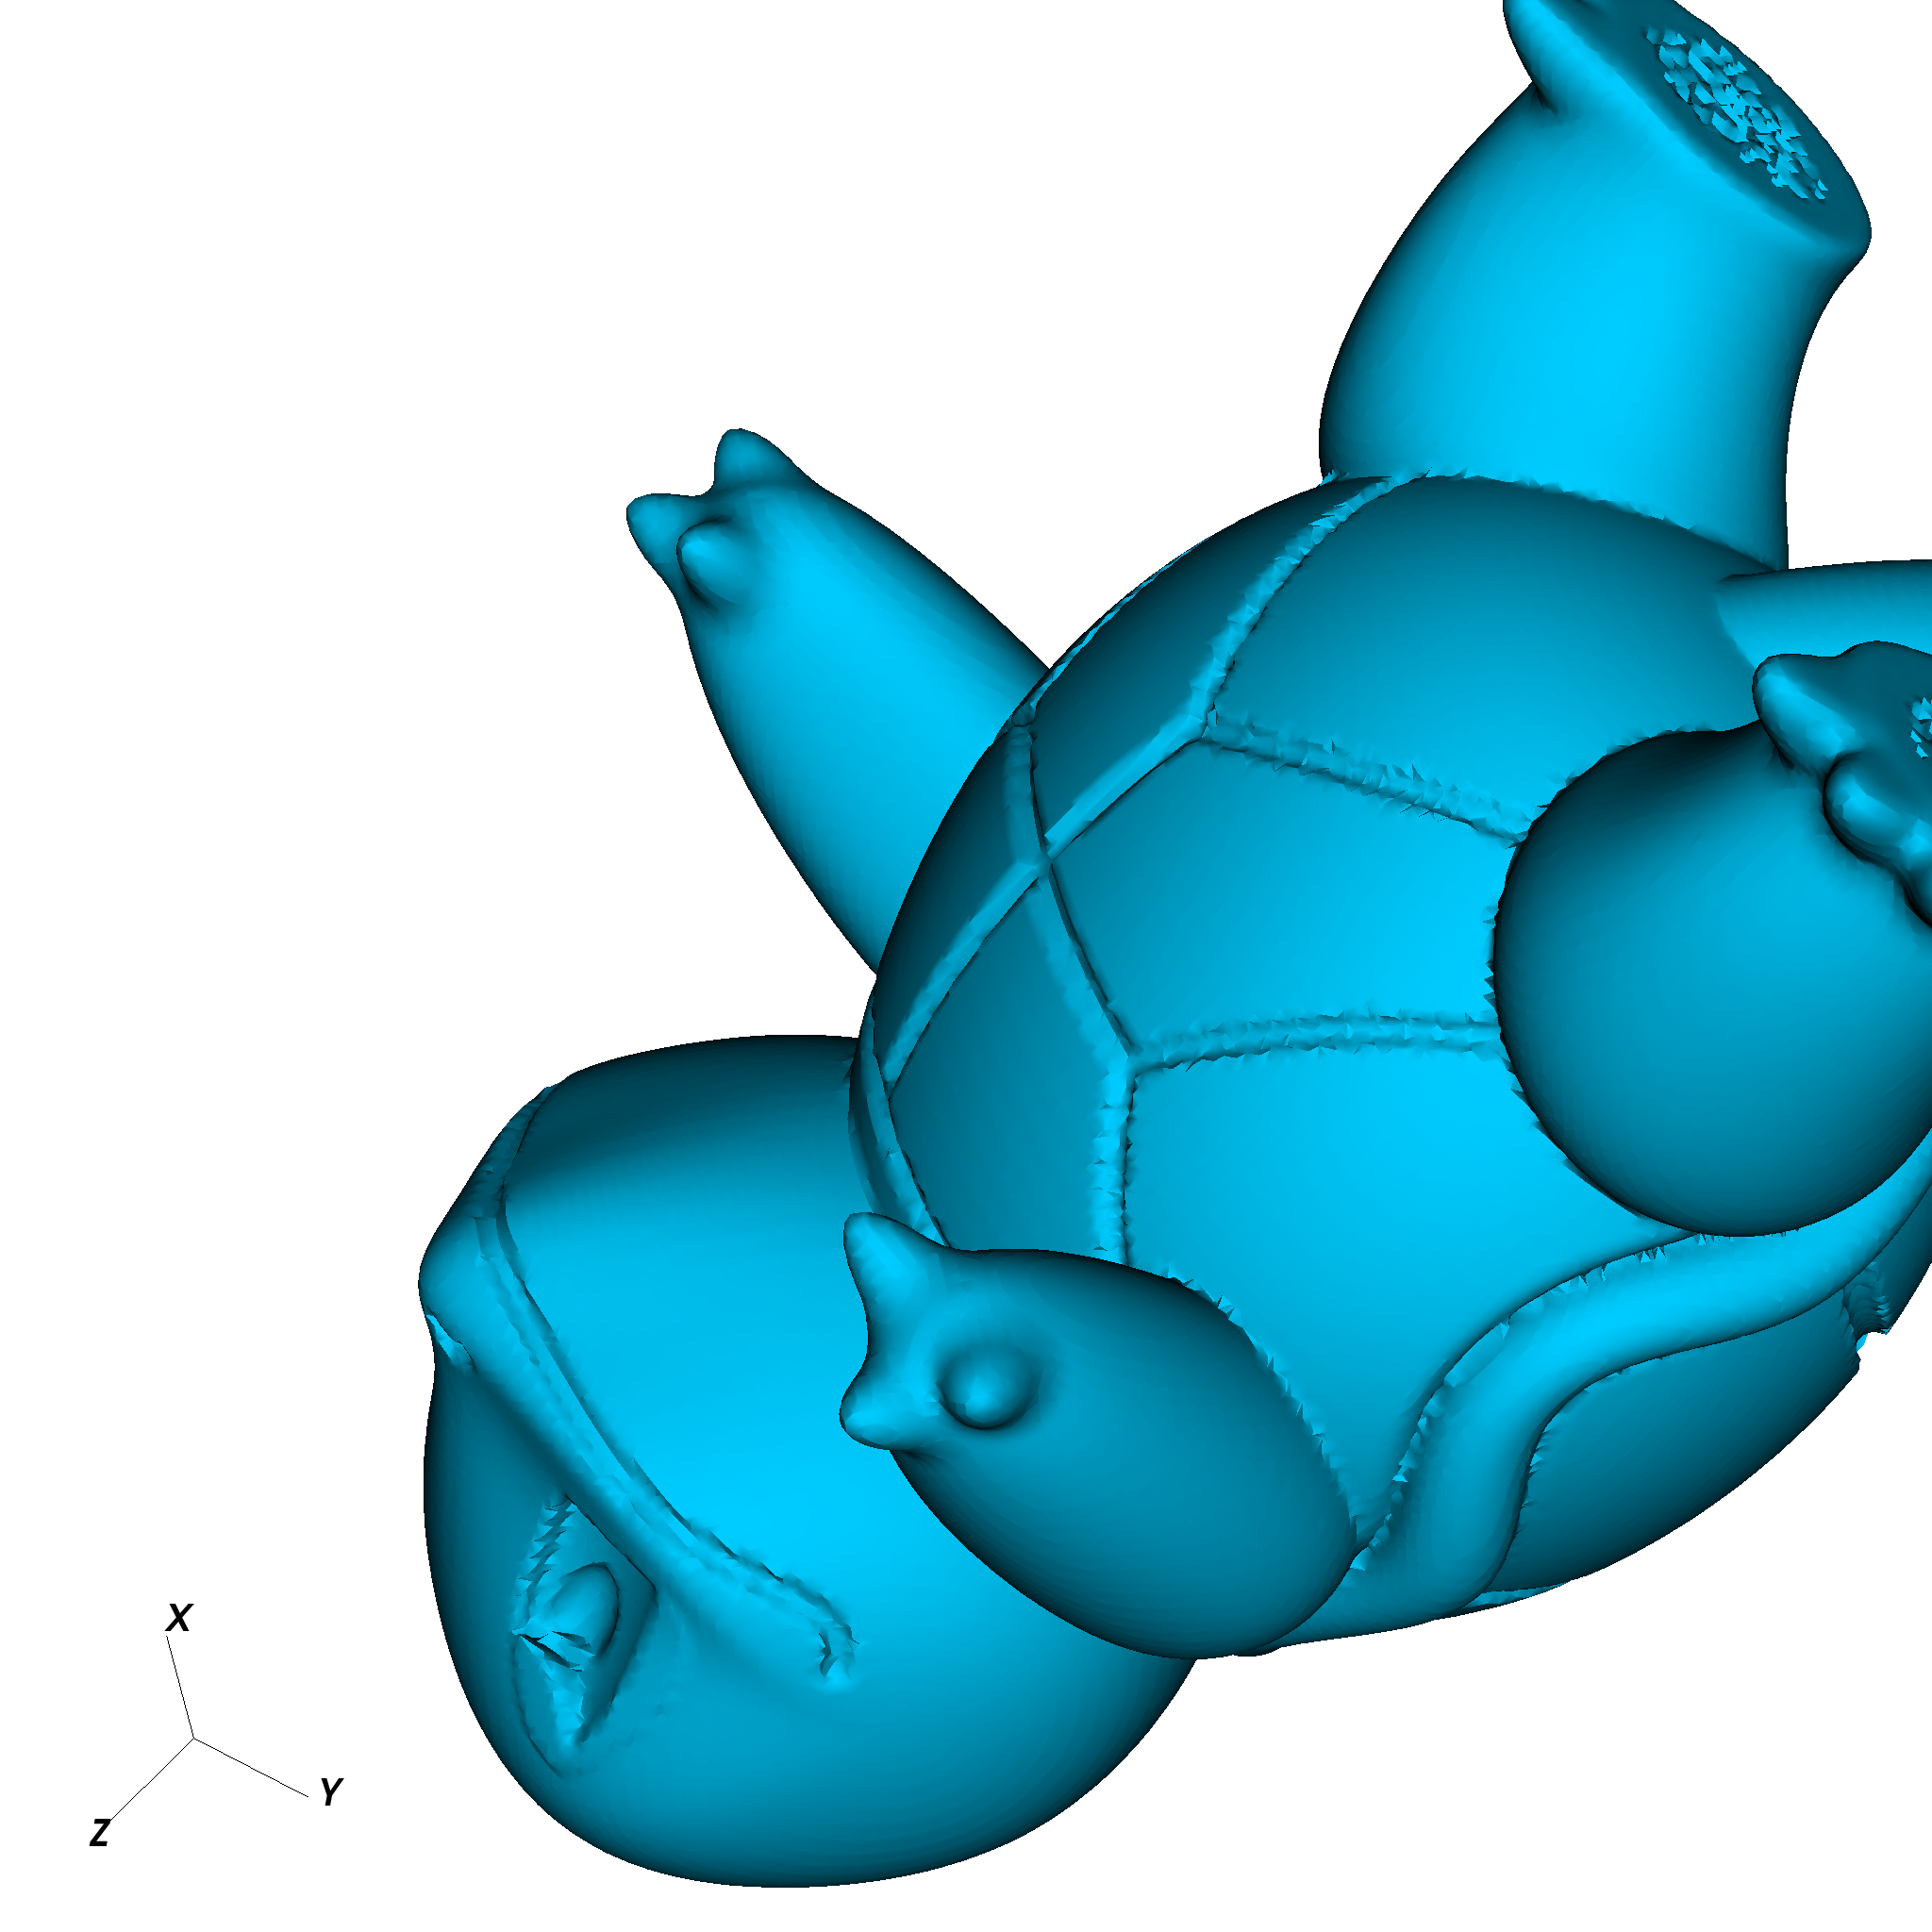
\includegraphics[width=\textwidth]{visit0021.png}
            \caption{}
            \label{ef4}
        \end{subfigure}
        \caption{The zero-level set of the signed distance function for the Squirtle STL sampled on a $240\times 320 \times 320$ mesh. There were $4\times 10^6$ marker particles seeded over the triangulated surface. The code ran in $\sim$2 minutes.}
        \label{SQ}
\end{figure*}

\begin{figure*}
\centering
        \begin{subfigure}[b]{0.475\textwidth}
            \centering
            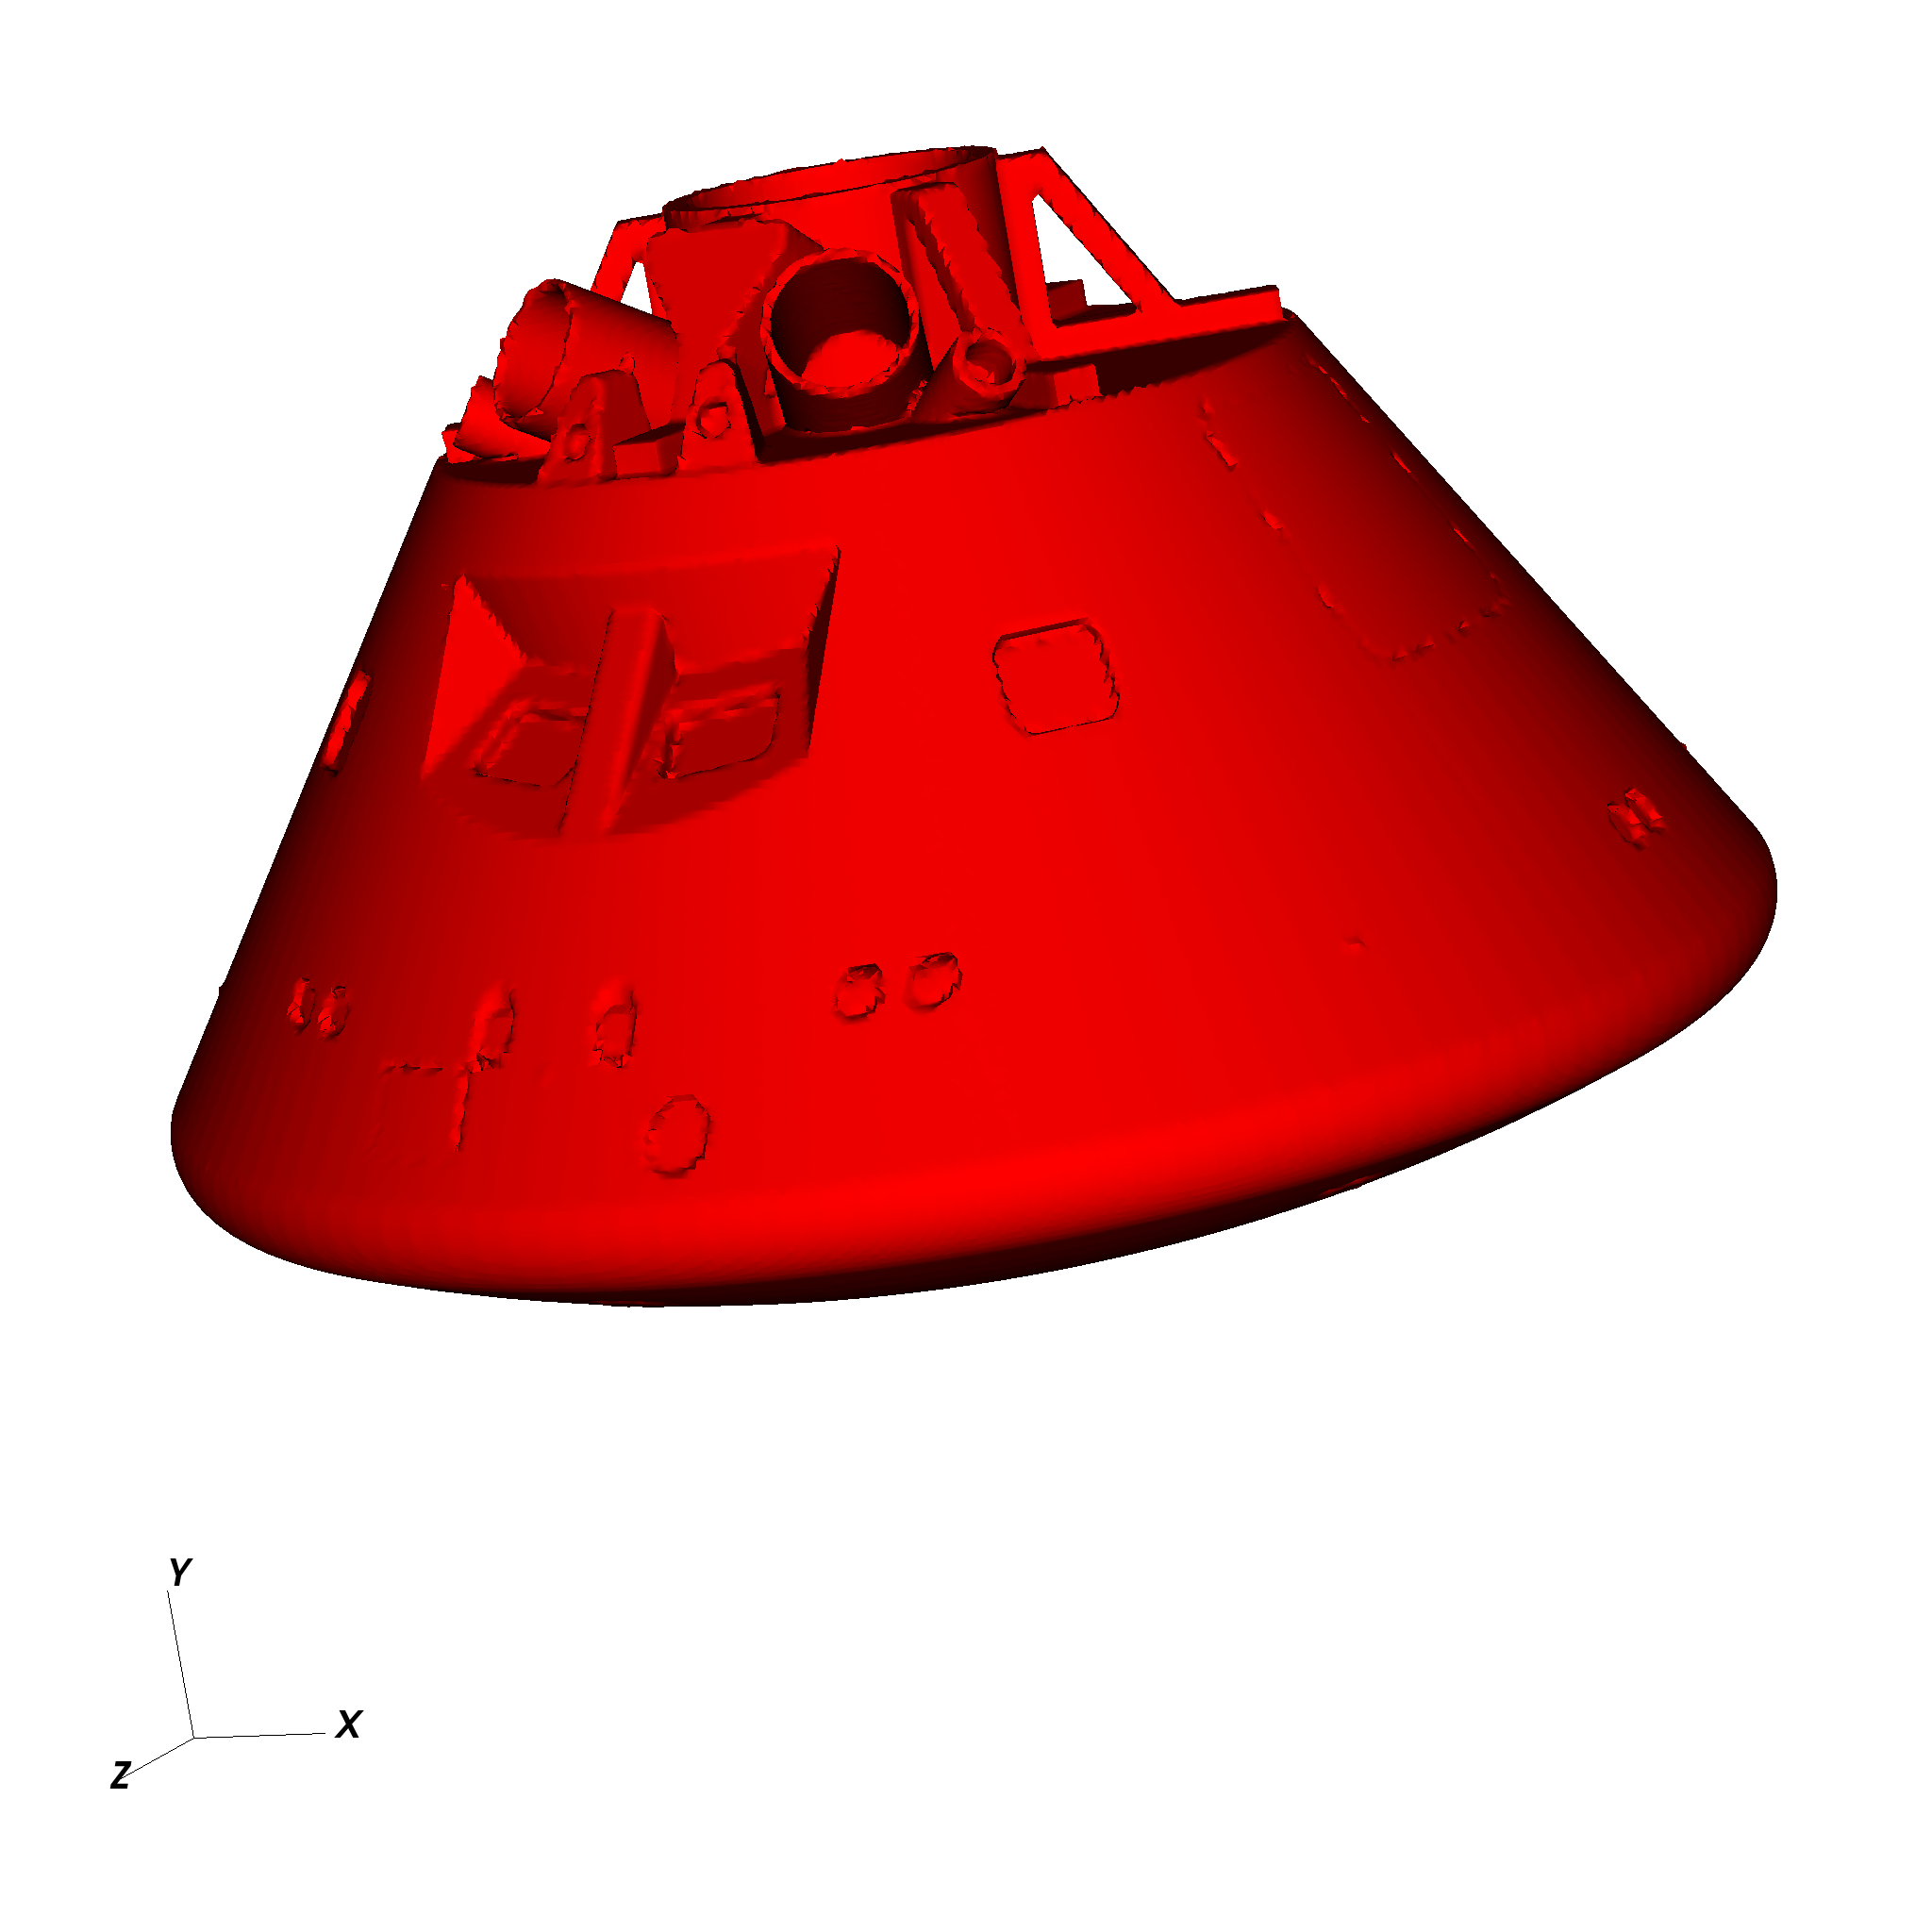
\includegraphics[width=\textwidth]{visit0003.png}
            \caption{}    
            \label{ef1}
        \end{subfigure}
        \hfill
        \begin{subfigure}[b]{0.475\textwidth}  
            \centering 
            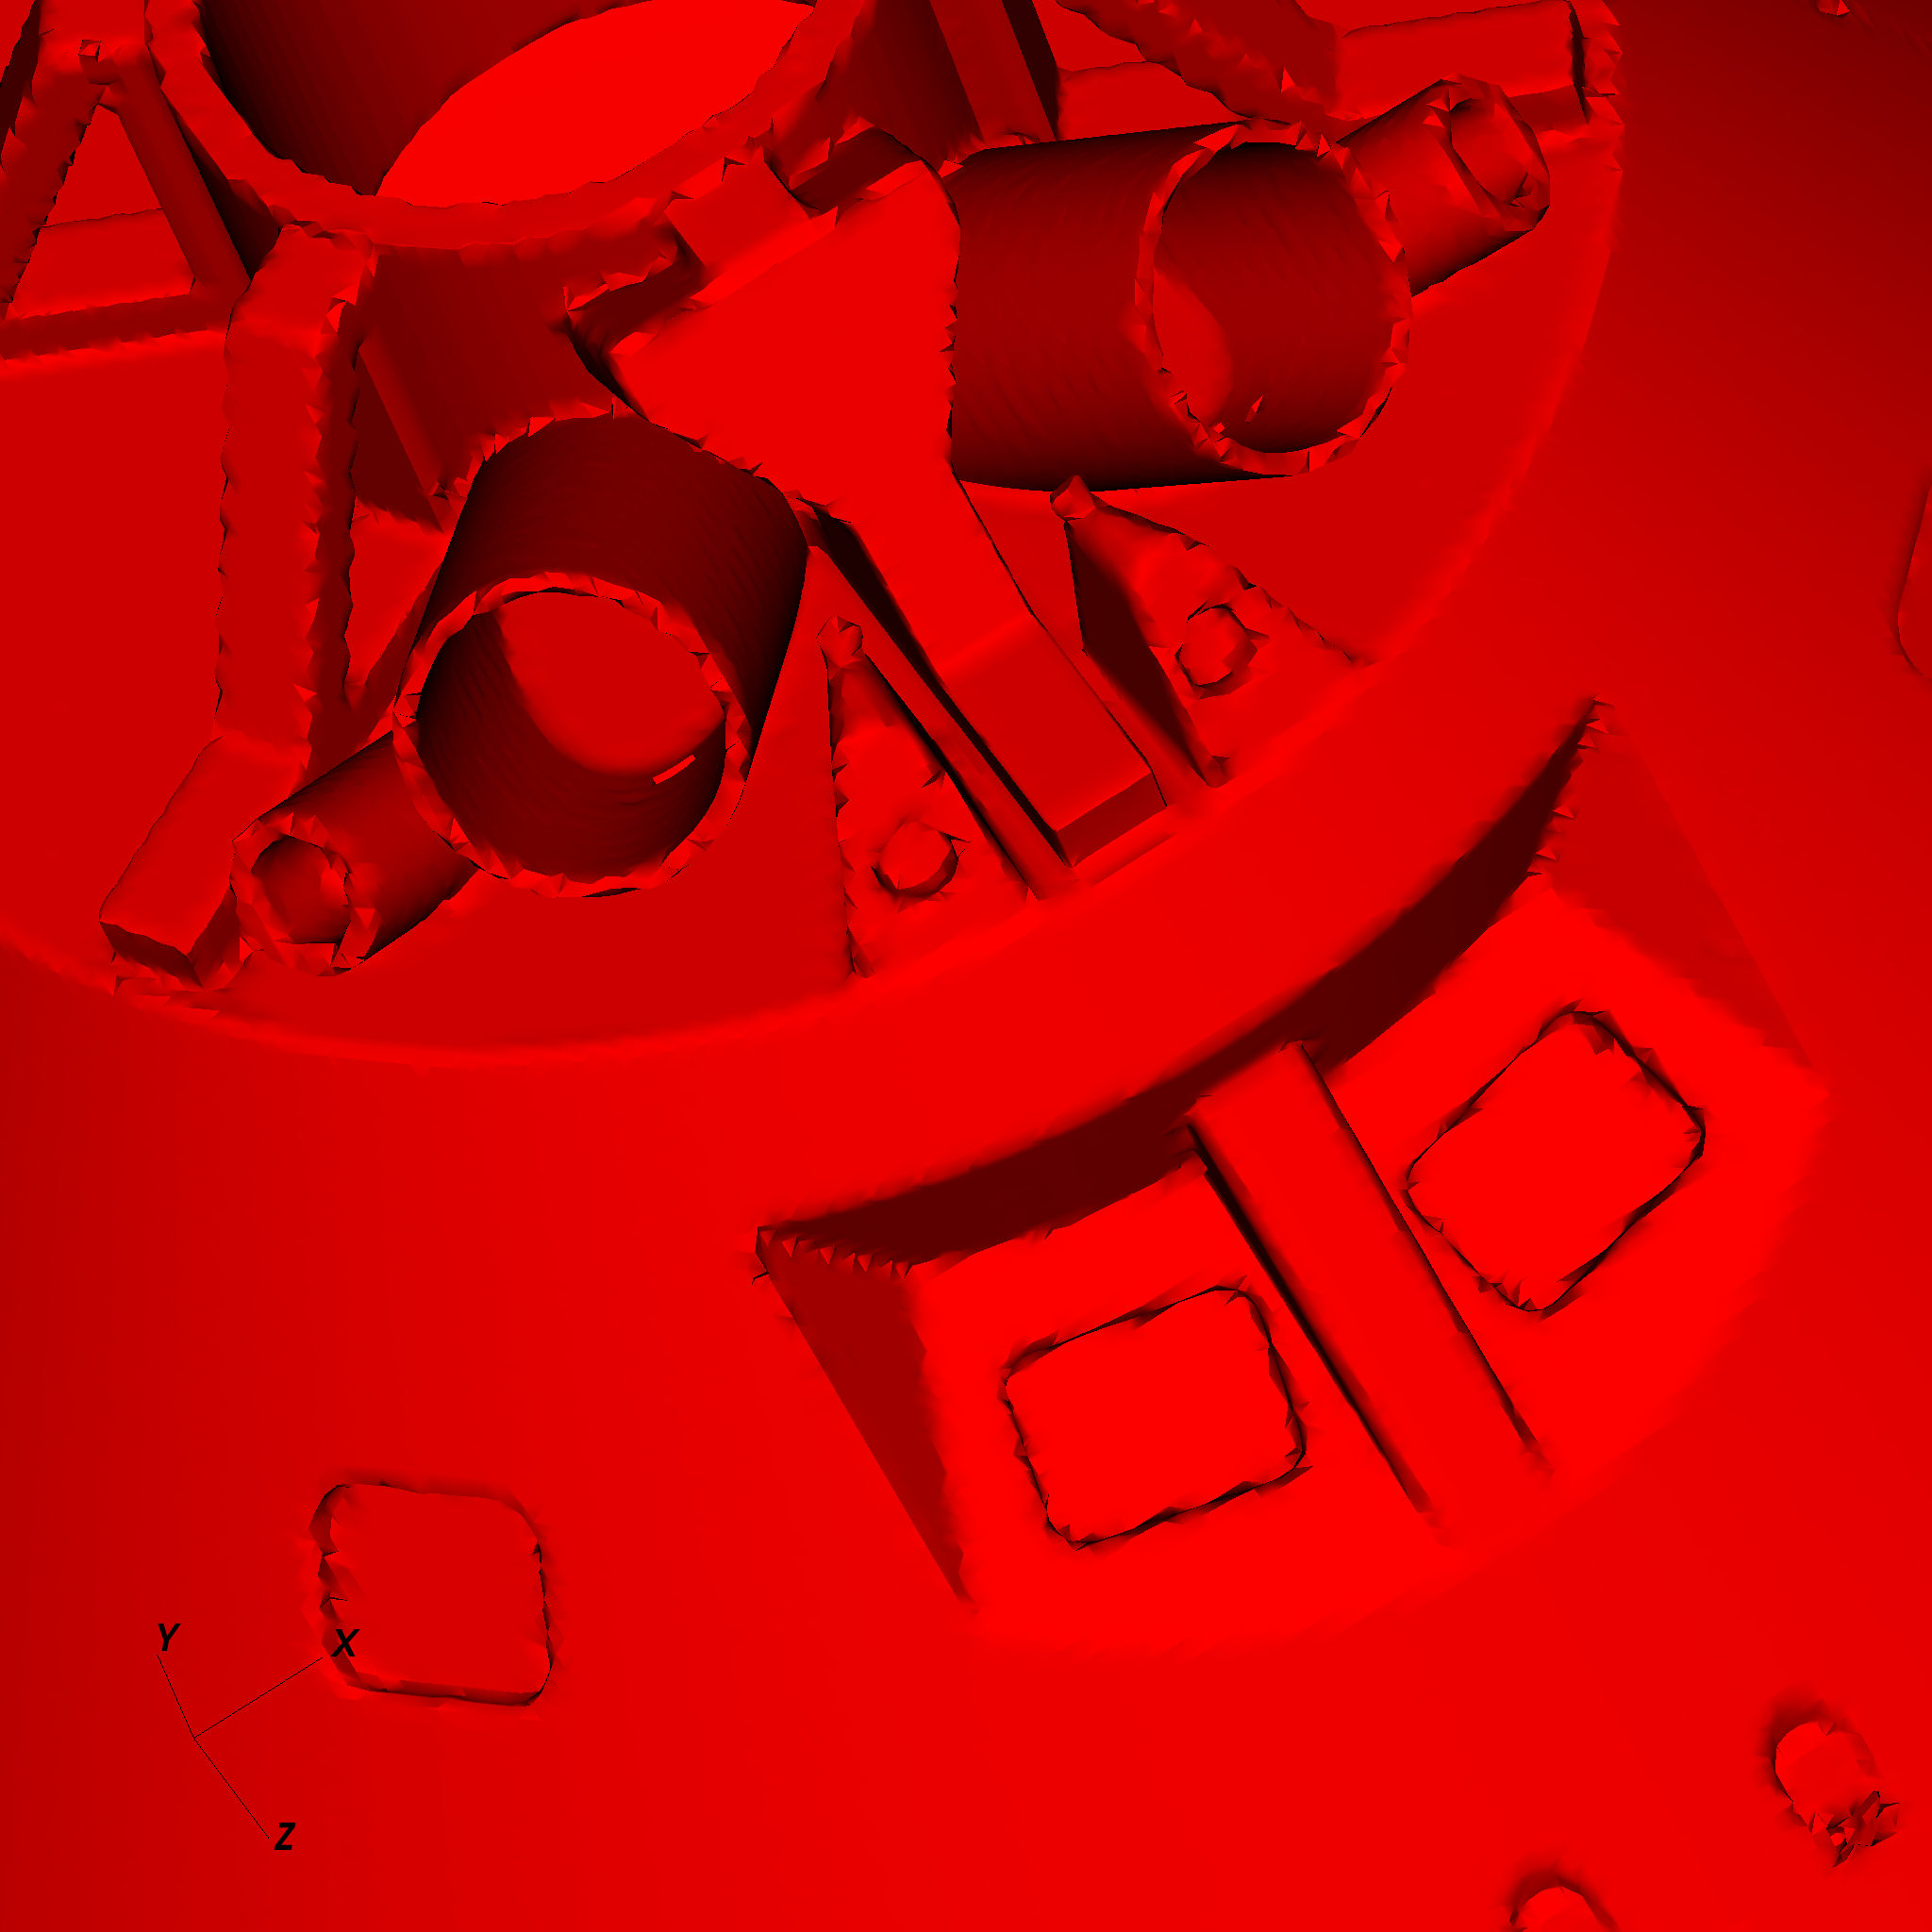
\includegraphics[width=\textwidth]{visit0000.png}
            \caption{}    
            \label{ef2}
        \end{subfigure}
        \vskip\baselineskip
        \begin{subfigure}[b]{0.475\textwidth}   
            \centering 
            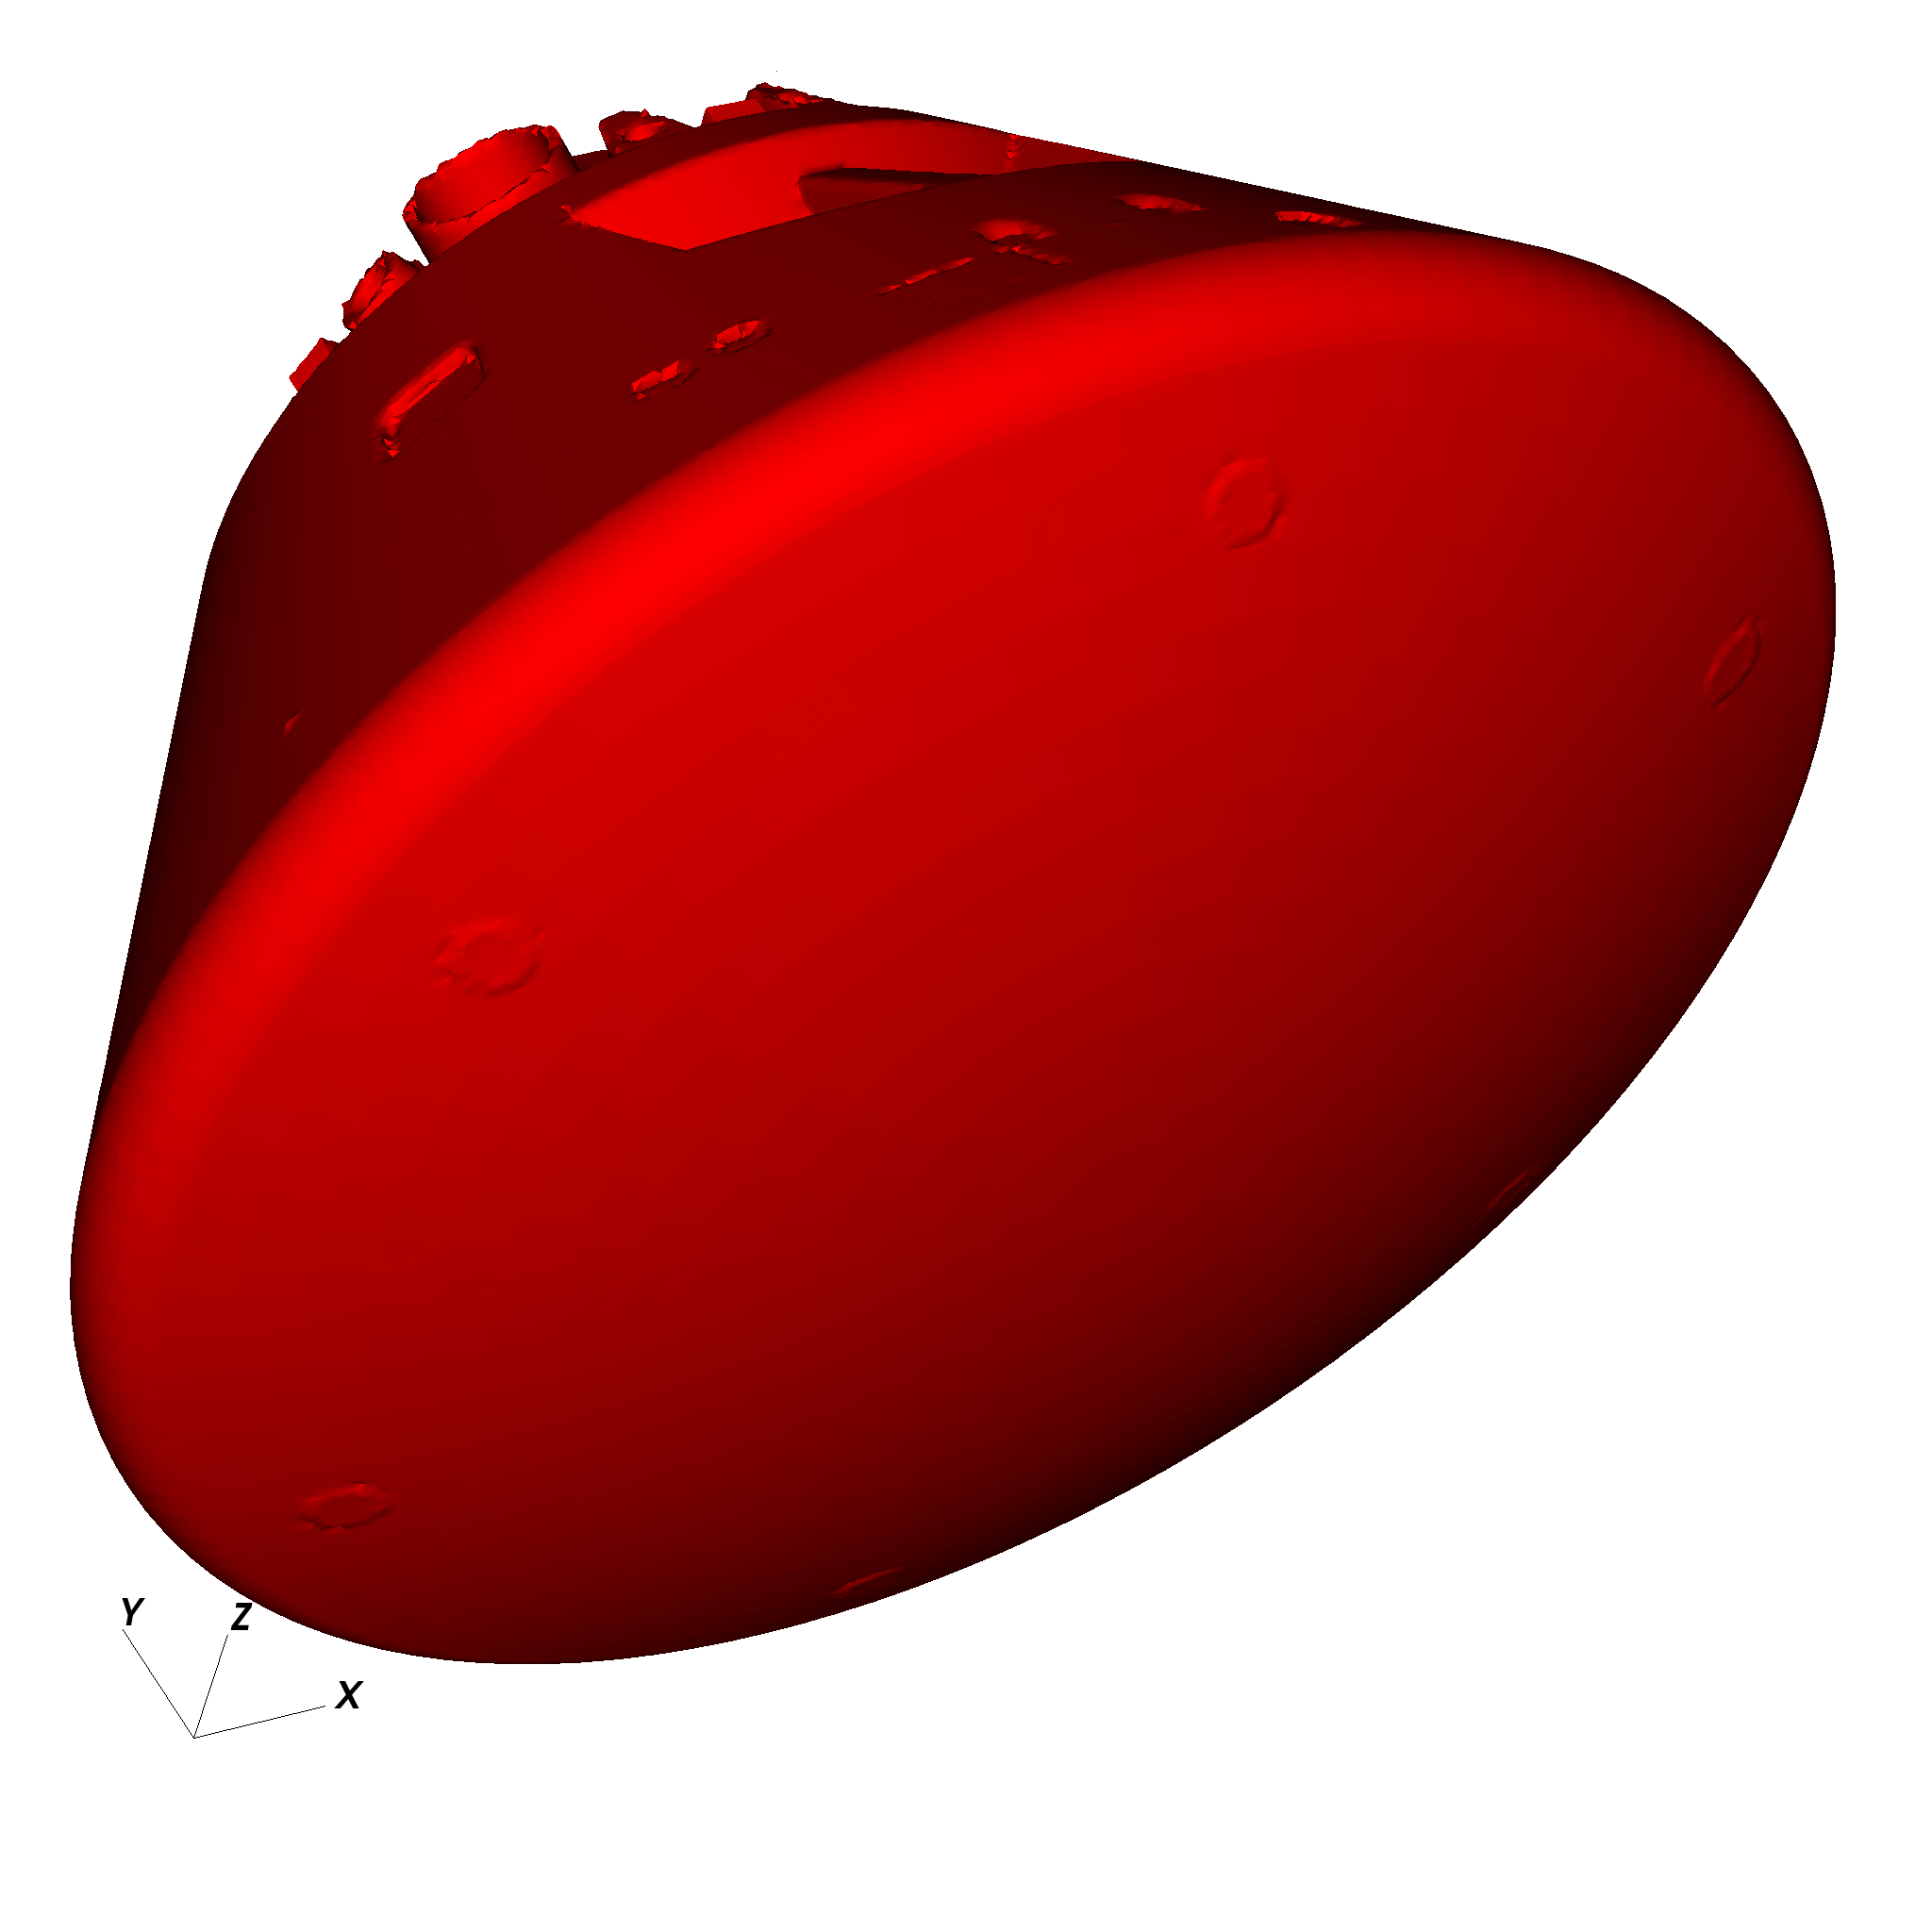
\includegraphics[width=\textwidth]{visit0001.png}
            \caption{}  
            \label{ef3}
        \end{subfigure}
        \quad
        \begin{subfigure}[b]{0.475\textwidth}   
            \centering 
            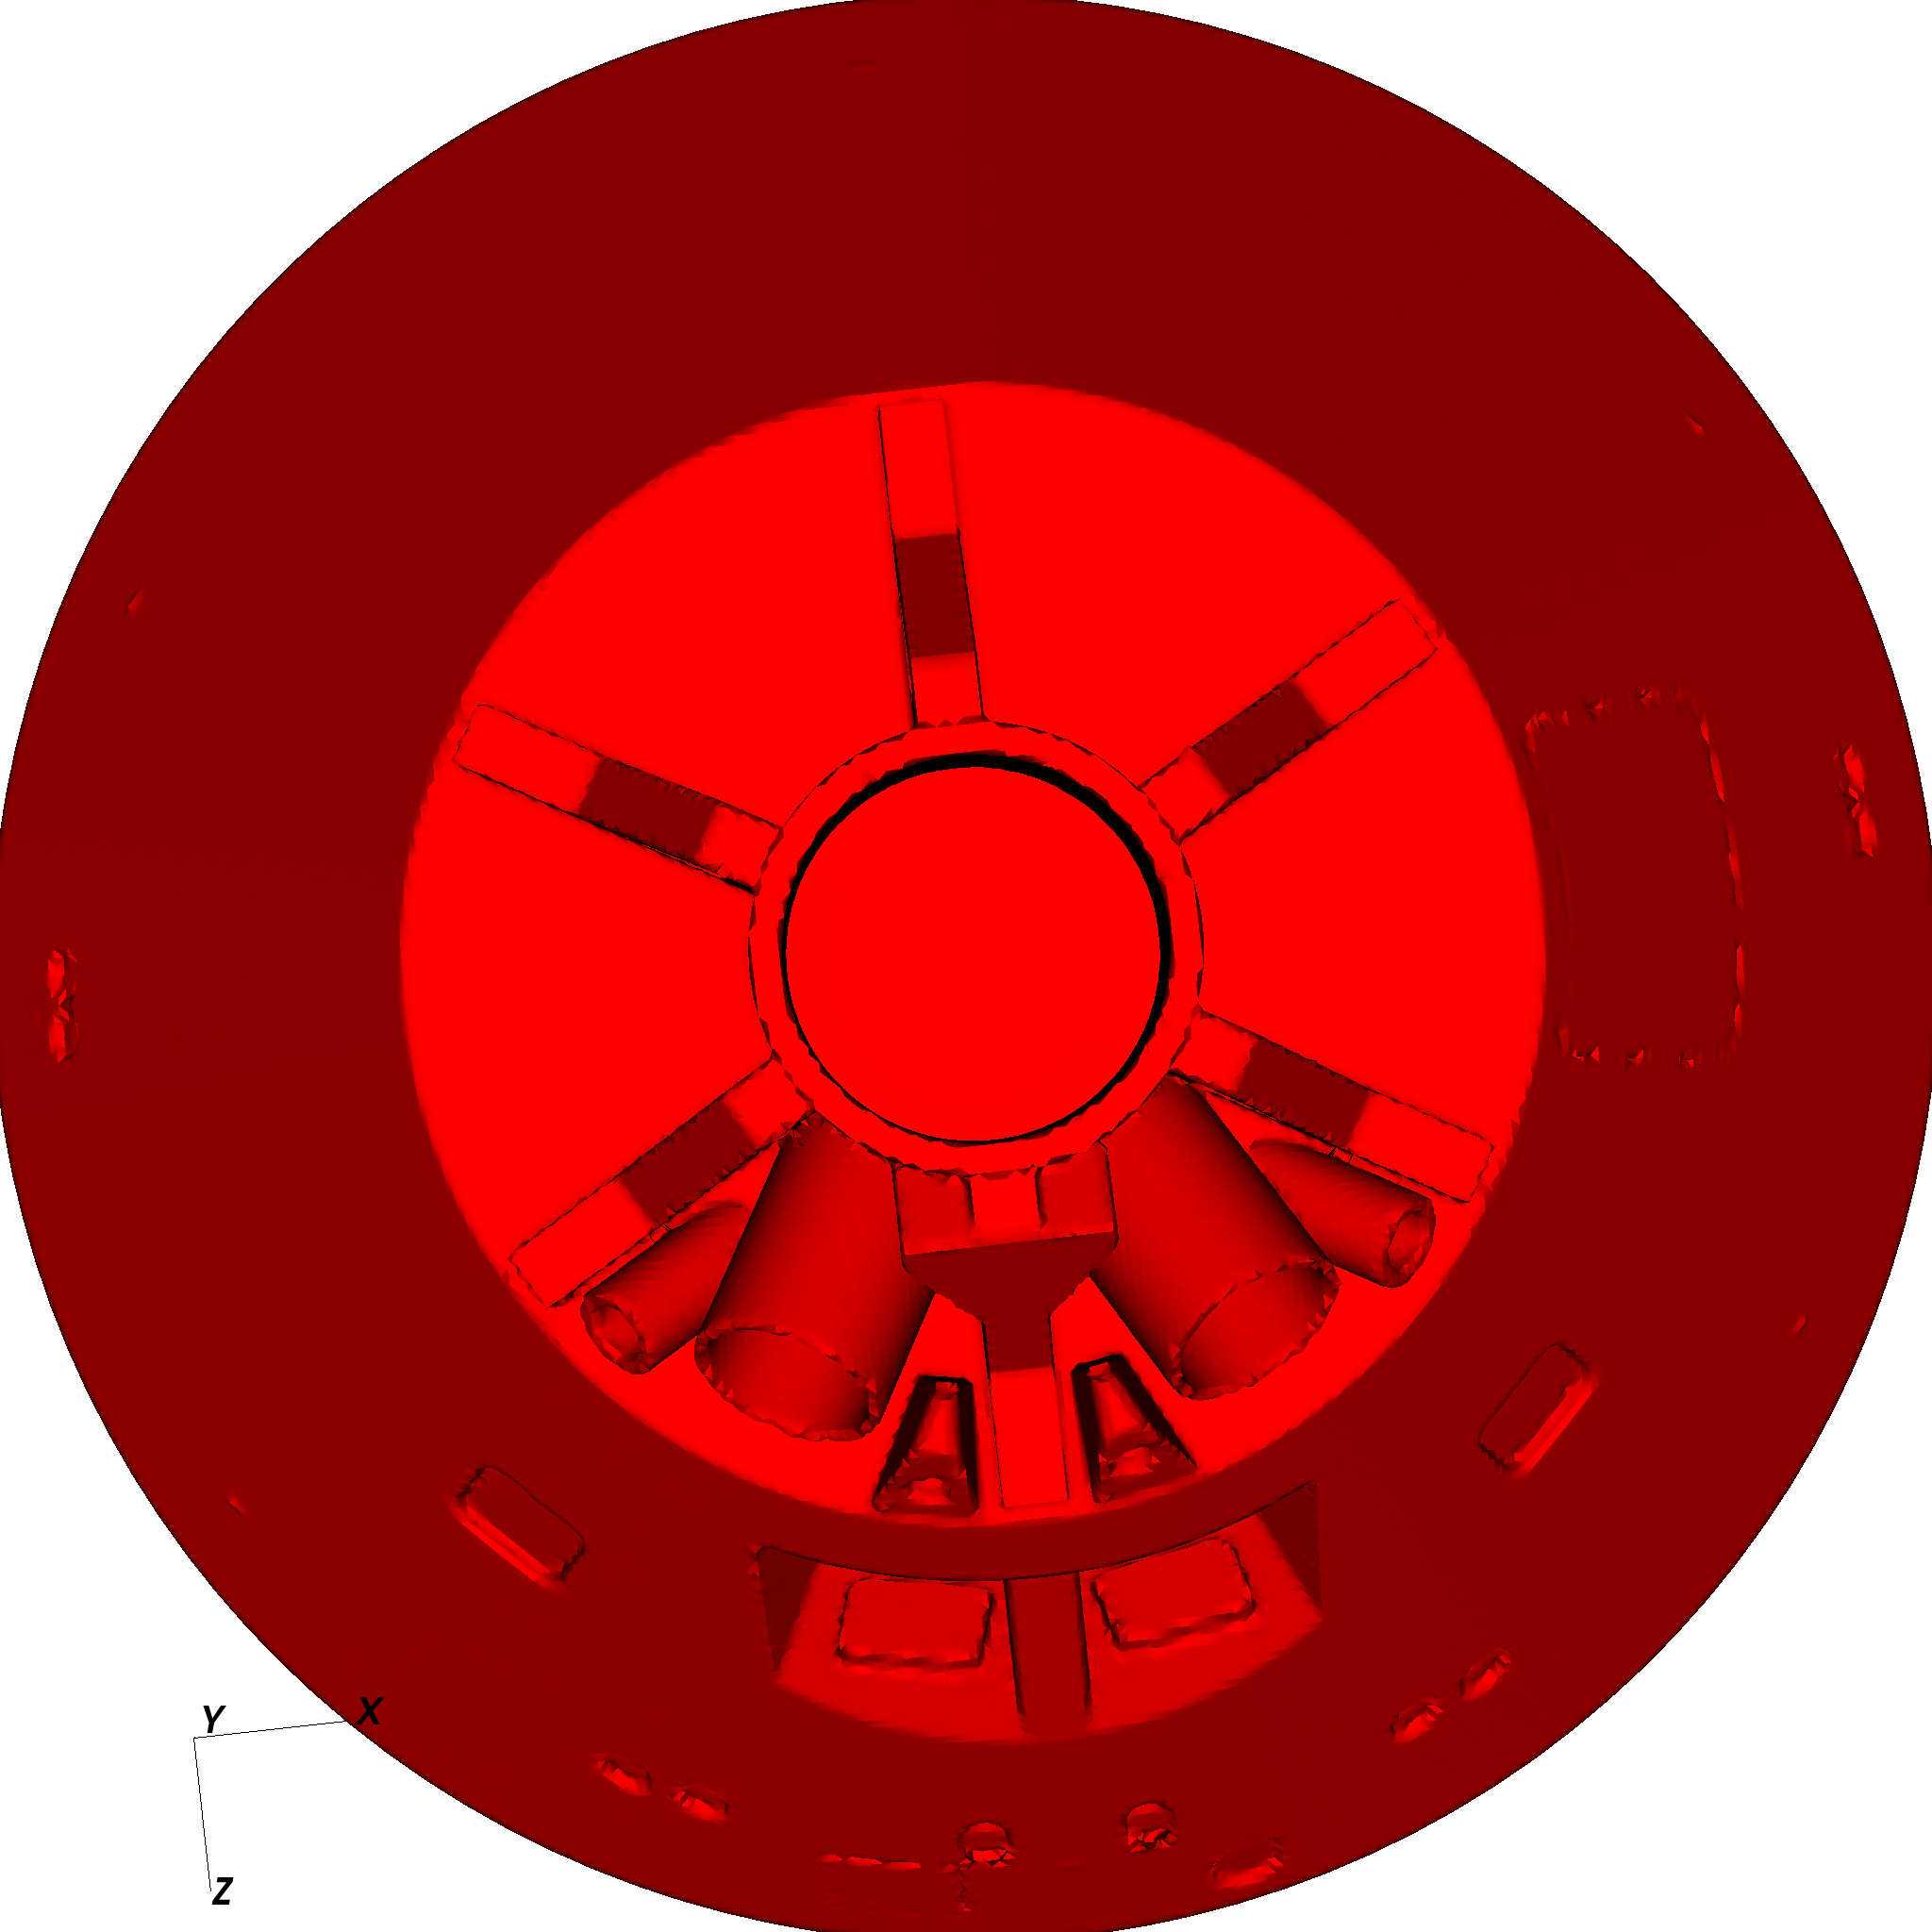
\includegraphics[width=\textwidth]{visit0002.png}
            \caption{}
            \label{ef4}
        \end{subfigure}
        \caption{The zero-level set of the signed distance function for the Orion capsule STL sampled on a $300^3$ mesh. There were $25\times 10^6$ marker particles seeded over the triangulated surface. The code ran in $\sim$10 minutes.}
        \label{SQ}
\end{figure*}


\FloatBarrier

\section{Conclusions and further work}

This study has shown that it is possible to use the APSS methodology to generate a
signed distance function from surface triangulation data. The method is fast, robust, 
and a single thread three-dimensional implementation requires $\sim$500 lines of C++ code.
There is much scope for further work to develop the capability of the method in handling
'bad' input data, and the method as implemented currently is prone to confusion when
the length scale of surface features is much smaller than the length scale of cells.
The following points describe how the work could be extended.

\begin{itemize}
\item The evaluation of $\phi$ throughout the grid using the APSS method is an embarrassingly parallel
problem. This method could be massively accelerated with relatively little effort, and should scale very well.
\item The weight function and the choice of which marker points to include in the computation of
$\phi(\textbf{x})$ are critical. It would be interesting to experiment with tighter weight functions-
even up to the limit that every sample point is computed from the single nearest marker particle (in this degenerate case the algebraic sphere becomes a plane).
\end{itemize}




\section*{References}

%\bibliographystyle{model3-num-names}
\bibliographystyle{plain}
\bibliography{./Mendeley.bib}




\end{document}

%%
%% End of file `elsarticle-template-3-num.tex'.